% Options for packages loaded elsewhere
\PassOptionsToPackage{unicode}{hyperref}
\PassOptionsToPackage{hyphens}{url}
\PassOptionsToPackage{dvipsnames,svgnames,x11names}{xcolor}
%
\documentclass[
  a4paper,
]{scrreport}

\usepackage{amsmath,amssymb}
\usepackage{lmodern}
\usepackage{iftex}
\ifPDFTeX
  \usepackage[T1]{fontenc}
  \usepackage[utf8]{inputenc}
  \usepackage{textcomp} % provide euro and other symbols
\else % if luatex or xetex
  \usepackage{unicode-math}
  \defaultfontfeatures{Scale=MatchLowercase}
  \defaultfontfeatures[\rmfamily]{Ligatures=TeX,Scale=1}
\fi
% Use upquote if available, for straight quotes in verbatim environments
\IfFileExists{upquote.sty}{\usepackage{upquote}}{}
\IfFileExists{microtype.sty}{% use microtype if available
  \usepackage[]{microtype}
  \UseMicrotypeSet[protrusion]{basicmath} % disable protrusion for tt fonts
}{}
\makeatletter
\@ifundefined{KOMAClassName}{% if non-KOMA class
  \IfFileExists{parskip.sty}{%
    \usepackage{parskip}
  }{% else
    \setlength{\parindent}{0pt}
    \setlength{\parskip}{6pt plus 2pt minus 1pt}}
}{% if KOMA class
  \KOMAoptions{parskip=half}}
\makeatother
\usepackage{xcolor}
\setlength{\emergencystretch}{3em} % prevent overfull lines
\setcounter{secnumdepth}{5}
% Make \paragraph and \subparagraph free-standing
\ifx\paragraph\undefined\else
  \let\oldparagraph\paragraph
  \renewcommand{\paragraph}[1]{\oldparagraph{#1}\mbox{}}
\fi
\ifx\subparagraph\undefined\else
  \let\oldsubparagraph\subparagraph
  \renewcommand{\subparagraph}[1]{\oldsubparagraph{#1}\mbox{}}
\fi

\usepackage{color}
\usepackage{fancyvrb}
\newcommand{\VerbBar}{|}
\newcommand{\VERB}{\Verb[commandchars=\\\{\}]}
\DefineVerbatimEnvironment{Highlighting}{Verbatim}{commandchars=\\\{\}}
% Add ',fontsize=\small' for more characters per line
\usepackage{framed}
\definecolor{shadecolor}{RGB}{241,243,245}
\newenvironment{Shaded}{\begin{snugshade}}{\end{snugshade}}
\newcommand{\AlertTok}[1]{\textcolor[rgb]{0.68,0.00,0.00}{#1}}
\newcommand{\AnnotationTok}[1]{\textcolor[rgb]{0.37,0.37,0.37}{#1}}
\newcommand{\AttributeTok}[1]{\textcolor[rgb]{0.40,0.45,0.13}{#1}}
\newcommand{\BaseNTok}[1]{\textcolor[rgb]{0.68,0.00,0.00}{#1}}
\newcommand{\BuiltInTok}[1]{\textcolor[rgb]{0.00,0.23,0.31}{#1}}
\newcommand{\CharTok}[1]{\textcolor[rgb]{0.13,0.47,0.30}{#1}}
\newcommand{\CommentTok}[1]{\textcolor[rgb]{0.37,0.37,0.37}{#1}}
\newcommand{\CommentVarTok}[1]{\textcolor[rgb]{0.37,0.37,0.37}{\textit{#1}}}
\newcommand{\ConstantTok}[1]{\textcolor[rgb]{0.56,0.35,0.01}{#1}}
\newcommand{\ControlFlowTok}[1]{\textcolor[rgb]{0.00,0.23,0.31}{#1}}
\newcommand{\DataTypeTok}[1]{\textcolor[rgb]{0.68,0.00,0.00}{#1}}
\newcommand{\DecValTok}[1]{\textcolor[rgb]{0.68,0.00,0.00}{#1}}
\newcommand{\DocumentationTok}[1]{\textcolor[rgb]{0.37,0.37,0.37}{\textit{#1}}}
\newcommand{\ErrorTok}[1]{\textcolor[rgb]{0.68,0.00,0.00}{#1}}
\newcommand{\ExtensionTok}[1]{\textcolor[rgb]{0.00,0.23,0.31}{#1}}
\newcommand{\FloatTok}[1]{\textcolor[rgb]{0.68,0.00,0.00}{#1}}
\newcommand{\FunctionTok}[1]{\textcolor[rgb]{0.28,0.35,0.67}{#1}}
\newcommand{\ImportTok}[1]{\textcolor[rgb]{0.00,0.46,0.62}{#1}}
\newcommand{\InformationTok}[1]{\textcolor[rgb]{0.37,0.37,0.37}{#1}}
\newcommand{\KeywordTok}[1]{\textcolor[rgb]{0.00,0.23,0.31}{#1}}
\newcommand{\NormalTok}[1]{\textcolor[rgb]{0.00,0.23,0.31}{#1}}
\newcommand{\OperatorTok}[1]{\textcolor[rgb]{0.37,0.37,0.37}{#1}}
\newcommand{\OtherTok}[1]{\textcolor[rgb]{0.00,0.23,0.31}{#1}}
\newcommand{\PreprocessorTok}[1]{\textcolor[rgb]{0.68,0.00,0.00}{#1}}
\newcommand{\RegionMarkerTok}[1]{\textcolor[rgb]{0.00,0.23,0.31}{#1}}
\newcommand{\SpecialCharTok}[1]{\textcolor[rgb]{0.37,0.37,0.37}{#1}}
\newcommand{\SpecialStringTok}[1]{\textcolor[rgb]{0.13,0.47,0.30}{#1}}
\newcommand{\StringTok}[1]{\textcolor[rgb]{0.13,0.47,0.30}{#1}}
\newcommand{\VariableTok}[1]{\textcolor[rgb]{0.07,0.07,0.07}{#1}}
\newcommand{\VerbatimStringTok}[1]{\textcolor[rgb]{0.13,0.47,0.30}{#1}}
\newcommand{\WarningTok}[1]{\textcolor[rgb]{0.37,0.37,0.37}{\textit{#1}}}

\providecommand{\tightlist}{%
  \setlength{\itemsep}{0pt}\setlength{\parskip}{0pt}}\usepackage{longtable,booktabs,array}
\usepackage{calc} % for calculating minipage widths
% Correct order of tables after \paragraph or \subparagraph
\usepackage{etoolbox}
\makeatletter
\patchcmd\longtable{\par}{\if@noskipsec\mbox{}\fi\par}{}{}
\makeatother
% Allow footnotes in longtable head/foot
\IfFileExists{footnotehyper.sty}{\usepackage{footnotehyper}}{\usepackage{footnote}}
\makesavenoteenv{longtable}
\usepackage{graphicx}
\makeatletter
\def\maxwidth{\ifdim\Gin@nat@width>\linewidth\linewidth\else\Gin@nat@width\fi}
\def\maxheight{\ifdim\Gin@nat@height>\textheight\textheight\else\Gin@nat@height\fi}
\makeatother
% Scale images if necessary, so that they will not overflow the page
% margins by default, and it is still possible to overwrite the defaults
% using explicit options in \includegraphics[width, height, ...]{}
\setkeys{Gin}{width=\maxwidth,height=\maxheight,keepaspectratio}
% Set default figure placement to htbp
\makeatletter
\def\fps@figure{htbp}
\makeatother

\usepackage{venndiagram}
\newcommand{\NN}{\mathbb{N}}
\newcommand{\ZZ}{\mathbb{Z}}
\newcommand{\QQ}{\mathbb{Q}}
\newcommand{\RR}{\mathbb{R}}
\newcommand{\CC}{\mathbb{C}}
\DeclareMathOperator{\operatorname{Int}}{Int}
\DeclareMathOperator{\operatorname{Ext}}{Ext}
\DeclareMathOperator{\operatorname{Fr}}{Fr}
\DeclareMathOperator{\Adh}{Adh}
\DeclareMathOperator{\Ac}{Ac}
\DeclareMathOperator{\sen}{sen}
\makeatletter
\@ifpackageloaded{tcolorbox}{}{\usepackage[many]{tcolorbox}}
\@ifpackageloaded{fontawesome5}{}{\usepackage{fontawesome5}}
\definecolor{quarto-callout-color}{HTML}{909090}
\definecolor{quarto-callout-note-color}{HTML}{0758E5}
\definecolor{quarto-callout-important-color}{HTML}{CC1914}
\definecolor{quarto-callout-warning-color}{HTML}{EB9113}
\definecolor{quarto-callout-tip-color}{HTML}{00A047}
\definecolor{quarto-callout-caution-color}{HTML}{FC5300}
\definecolor{quarto-callout-color-frame}{HTML}{acacac}
\definecolor{quarto-callout-note-color-frame}{HTML}{4582ec}
\definecolor{quarto-callout-important-color-frame}{HTML}{d9534f}
\definecolor{quarto-callout-warning-color-frame}{HTML}{f0ad4e}
\definecolor{quarto-callout-tip-color-frame}{HTML}{02b875}
\definecolor{quarto-callout-caution-color-frame}{HTML}{fd7e14}
\makeatother
\makeatletter
\@ifpackageloaded{tikz}{}{\usepackage{tikz}}
\makeatother
\makeatletter
\@ifpackageloaded{bookmark}{}{\usepackage{bookmark}}
\makeatother
\makeatletter
\@ifpackageloaded{caption}{}{\usepackage{caption}}
\AtBeginDocument{%
\ifdefined\contentsname
  \renewcommand*\contentsname{Indice de contenidos}
\else
  \newcommand\contentsname{Indice de contenidos}
\fi
\ifdefined\listfigurename
  \renewcommand*\listfigurename{Listado de Figuras}
\else
  \newcommand\listfigurename{Listado de Figuras}
\fi
\ifdefined\listtablename
  \renewcommand*\listtablename{Listado de Tablas}
\else
  \newcommand\listtablename{Listado de Tablas}
\fi
\ifdefined\figurename
  \renewcommand*\figurename{Figura}
\else
  \newcommand\figurename{Figura}
\fi
\ifdefined\tablename
  \renewcommand*\tablename{Tabla}
\else
  \newcommand\tablename{Tabla}
\fi
}
\@ifpackageloaded{float}{}{\usepackage{float}}
\floatstyle{ruled}
\@ifundefined{c@chapter}{\newfloat{codelisting}{h}{lop}}{\newfloat{codelisting}{h}{lop}[chapter]}
\floatname{codelisting}{Listado}
\newcommand*\listoflistings{\listof{codelisting}{Listado de Listatdos}}
\usepackage{amsthm}
\theoremstyle{definition}
\newtheorem{exercise}{Ejercicio}[chapter]
\theoremstyle{remark}
\renewcommand*{\proofname}{Prueba}
\newtheorem*{remark}{Observación}
\newtheorem*{solution}{Solución}
\makeatother
\makeatletter
\@ifpackageloaded{caption}{}{\usepackage{caption}}
\@ifpackageloaded{subcaption}{}{\usepackage{subcaption}}
\makeatother
\makeatletter
\@ifpackageloaded{tcolorbox}{}{\usepackage[many]{tcolorbox}}
\makeatother
\makeatletter
\@ifundefined{shadecolor}{\definecolor{shadecolor}{rgb}{.97, .97, .97}}
\makeatother
\makeatletter
\makeatother
\ifLuaTeX
\usepackage[bidi=basic]{babel}
\else
\usepackage[bidi=default]{babel}
\fi
\babelprovide[main,import]{spanish}
% get rid of language-specific shorthands (see #6817):
\let\LanguageShortHands\languageshorthands
\def\languageshorthands#1{}
\ifLuaTeX
  \usepackage{selnolig}  % disable illegal ligatures
\fi
\IfFileExists{bookmark.sty}{\usepackage{bookmark}}{\usepackage{hyperref}}
\IfFileExists{xurl.sty}{\usepackage{xurl}}{} % add URL line breaks if available
\urlstyle{same} % disable monospaced font for URLs
\hypersetup{
  pdftitle={Pácticas de Análisis Matemático con Julia},
  pdfauthor={Alfredo Sánchez Alberca},
  pdflang={es},
  colorlinks=true,
  linkcolor={blue},
  filecolor={Maroon},
  citecolor={Blue},
  urlcolor={Blue},
  pdfcreator={LaTeX via pandoc}}

\title{Pácticas de Análisis Matemático con Julia}
\author{Alfredo Sánchez Alberca}
\date{1/6/2022}

\begin{document}
\begin{titlepage}

%\AddToShipoutPicture*{\put(0,0){\includegraphics[scale=0.8]{img/background2}}} % Imagen de fondo, requiere el paquete eso-pic.
\begin{center}
\vspace*{5cm}

\Huge
{\textbf{\textsf{Pácticas de Análisis Matemático con Julia}}}

\vspace{0.5cm}
\LARGE
{\textbf{\textsf{}}}

\vspace{1.5cm}


\includegraphics[width=0.4\textwidth]{img/logos/infinito-julia.png}
\end{center}

\vfill

\begin{flushleft}
\begin{tabular}{ll}

\includegraphics[width=0.1\textwidth]{img/logos/aprendeconalf.png} & \parbox[b]{5cm}{\Large\textsf{Alfredo
Sánchez
Alberca}\\ \textsf{asalber@ceu.es} \\ \textsf{https://aprendeconalf.es}}
\end{tabular}
\end{flushleft}
\end{titlepage}\ifdefined\Shaded\renewenvironment{Shaded}{\begin{tcolorbox}[interior hidden, borderline west={3pt}{0pt}{shadecolor}, enhanced, breakable, sharp corners, boxrule=0pt, frame hidden]}{\end{tcolorbox}}\fi

\renewcommand*\contentsname{Indice de contenidos}
{
\hypersetup{linkcolor=}
\setcounter{tocdepth}{2}
\tableofcontents
}
\bookmarksetup{startatroot}

\hypertarget{prefacio}{%
\chapter*{Prefacio}\label{prefacio}}
\addcontentsline{toc}{chapter}{Prefacio}

¡Bienvenido a Prácticas de Análisis Matemático con Julia!

Este libro presenta una recopilación de prácticas de Análisis Matemático
en una y varias variables reales con el lenguaje de programación
\href{https://julialang.org/}{Julia}, con problemas aplicados a las
Ciencias y las Ingenierías.

No es un libro para aprender a programar con Julia, ya que solo enseña
el uso del lenguaje y de algunos de sus paquetes para resolver problemas
de Cálculo tanto numérico como simbólico. Para quienes estén interesados
en aprender a programar en este Julia, os recomiendo leer este
\href{https://aprendeconalf.es/manual-julia/}{manual de Julia}.

\hypertarget{licencia}{%
\section*{Licencia}\label{licencia}}
\addcontentsline{toc}{section}{Licencia}

Esta obra está bajo una licencia Reconocimiento -- No comercial --
Compartir bajo la misma licencia 3.0 España de Creative Commons. Para
ver una copia de esta licencia, visite
\url{https://creativecommons.org/licenses/by-nc-sa/3.0/es/}.

Con esta licencia eres libre de:

\begin{itemize}
\tightlist
\item
  Copiar, distribuir y mostrar este trabajo.
\item
  Realizar modificaciones de este trabajo.
\end{itemize}

Bajo las siguientes condiciones:

\begin{itemize}
\item
  \textbf{Reconocimiento}. Debe reconocer los créditos de la obra de la
  manera especificada por el autor o el licenciador (pero no de una
  manera que sugiera que tiene su apoyo o apoyan el uso que hace de su
  obra).
\item
  \textbf{No comercial}. No puede utilizar esta obra para fines
  comerciales.
\item
  \textbf{Compartir bajo la misma licencia}. Si altera o transforma esta
  obra, o genera una obra derivada, sólo puede distribuir la obra
  generada bajo una licencia idéntica a ésta.
\end{itemize}

Al reutilizar o distribuir la obra, tiene que dejar bien claro los
términos de la licencia de esta obra.

Estas condiciones pueden no aplicarse si se obtiene el permiso del
titular de los derechos de autor.

Nada en esta licencia menoscaba o restringe los derechos morales del
autor.

\bookmarksetup{startatroot}

\hypertarget{introducciuxf3n}{%
\chapter{Introducción}\label{introducciuxf3n}}

La gran potencia de cálculo alcanzada por los ordenadores en las últimas
décadas ha convertido a los mismos en poderosas herramientas al servicio
de todas aquellas disciplinas que, como las matemáticas, requieren
cálculos largos y complejos.

\href{https://julialang.org/}{Julia} es un lenguaje de programación
especialmente orientado al cálculo numérico y el análisis de datos.
Julia permite además realizar cálculos simbólicos y dispone de una gran
\href{https://julialang.org/packages/}{biblioteca de paquetes} con
aplicaciones en muy diversas áreas de las Matemáticas como Cálculo,
Álgebra, Geometría, Matemática Discreta o Estadística.


\includegraphics{./img/logos/logo-julia.png}

La ventaja de Julia frente a otros programas habituales de cálculo como
Mathematica, MATLAB o Sage radica en su potencia de cálculo y su
velocidad (equiparable al lenguaje C), lo que lo hace ideal para manejar
grandes volúmenes de datos o realizar tareas que requieran largos y
complejos cálculos. Además, es software libre por lo que resulta ideal
para introducirlo en el aula como soporte computacional para los modelos
matemáticos sin coste alguno.

En el siguiente enlace se explica el procedimiento de
\href{https://aprendeconalf.es/manual-julia/intro.html\#instalaci\%C3\%B3n-de-julia}{instalación
de Julia}.

Existen también varios entornos de desarrollo online que permiten
ejecutar código en Julia sin necesidad de instalarlo en nuestro
ordenador, como por ejemplo
\href{https://replit.com/languages/julia}{Replit},
\href{https://cocalc.com/}{Cocalc} o
\href{https://codeanywhere.com/languages/julia}{Codeanywhere}.

El objetivo de esta práctica es introducir al alumno en la utilización
de este lenguaje, enseñándole a realizar las operaciones básicas más
habituales en Cálculo.

\hypertarget{el-repl-de-julia}{%
\section{El REPL de Julia}\label{el-repl-de-julia}}

Para arrancar el REPL\^{}(REPL es el acrónimo de Read, Evaluate, Print
and Loop, que describe el funcionamiento del compilador de Julia) de
julia basta con abrir una terminal y teclear \texttt{julia}.

\begin{Shaded}
\begin{Highlighting}[]
\NormalTok{prompt}\OperatorTok{\textgreater{}}\NormalTok{ julia}
\NormalTok{               \_}
\NormalTok{   \_       \_ }\FunctionTok{\_}\NormalTok{(\_)\_     }\OperatorTok{|}\NormalTok{  Documentation}\OperatorTok{:}\NormalTok{ https}\OperatorTok{://}\NormalTok{docs.julialang.org}
\NormalTok{  (\_)     }\OperatorTok{|}\NormalTok{ (\_) (\_)    }\OperatorTok{|}
\NormalTok{   \_ \_   \_}\OperatorTok{|} \OperatorTok{|}\NormalTok{\_  \_\_ \_   }\OperatorTok{|}  \DataTypeTok{Type} \StringTok{"?"} \ControlFlowTok{for}\NormalTok{ help, }\StringTok{"]?"} \ControlFlowTok{for} \BuiltInTok{Pkg}\NormalTok{ help.}
  \OperatorTok{|} \OperatorTok{|} \OperatorTok{|} \OperatorTok{|} \OperatorTok{|} \OperatorTok{|} \OperatorTok{|/}\NormalTok{ \_}\SpecialStringTok{\textasciigrave{} |  |}
  \OperatorTok{|} \OperatorTok{|} \OperatorTok{|}\NormalTok{\_}\OperatorTok{|} \OperatorTok{|} \OperatorTok{|} \OperatorTok{|}\NormalTok{ (\_}\OperatorTok{|} \OperatorTok{|}  \OperatorTok{|}\NormalTok{  Version }\FloatTok{1.7.3}\NormalTok{ (}\FloatTok{2022}\OperatorTok{{-}}\FloatTok{05}\OperatorTok{{-}}\FloatTok{06}\NormalTok{)}
\NormalTok{ \_}\OperatorTok{/} \OperatorTok{|\textbackslash{}}\NormalTok{\_\_}\CharTok{\textquotesingle{}\_|\_|\_|\textbackslash{}\_\_\textquotesingle{}}\NormalTok{\_}\OperatorTok{|}  \OperatorTok{|}\NormalTok{  Official https}\OperatorTok{://}\NormalTok{julialang.org}\OperatorTok{/}\NormalTok{ release}
\OperatorTok{|}\NormalTok{\_\_}\OperatorTok{/}                   \OperatorTok{|}

\NormalTok{julia}\OperatorTok{\textgreater{}}
\end{Highlighting}
\end{Shaded}

\hypertarget{el-gestor-de-paquetes-de-julia}{%
\section{El gestor de paquetes de
Julia}\label{el-gestor-de-paquetes-de-julia}}

Julia viene con varios paquetes básicos preinstalados, como por ejemplo
el paquete \texttt{LinearAlgebra} que define funciones básicas del
Álgebra Lineal, pero en estas prácticas utilizaremos otros muchos
paquetes que añaden más funcionalidades que no vienen instalados por
defecto y tendremos que instalarlos aparte. Julia tiene un potente
gestor de paquetes que facilita la búsqueda, instalación, actualización
y eliminación de paquetes.

Por defecto el gestor de paquetes utiliza el
\href{https://julialang.org/packages/}{repositorio de paquetes oficial}
pero se pueden instalar paquetes de otros repositorios.

Para entrar en el modo de gestión de paquetes hay que teclear
\texttt{{]}}. Esto produce un cambio en el \emph{prompt} del REPL de
Julia.

Los comandos más habituales son:

\begin{itemize}
\tightlist
\item
  \texttt{add\ p}: Instala el paquete \texttt{p} en el entorno activo de
  Julia.
\item
  \texttt{update}: Actualiza los paquetes del entorno activo de Julia.
\item
  \texttt{status}: Muestra los paquetes instalados y sus versiones en el
  entorno activo de Julia.
\item
  \texttt{remove\ p}: Elimina el paquete \texttt{p} del entorno activo
  de Julia.
\end{itemize}

\begin{tcolorbox}[enhanced jigsaw, arc=.35mm, toptitle=1mm, toprule=.15mm, breakable, colframe=quarto-callout-note-color-frame, bottomtitle=1mm, titlerule=0mm, title=\textcolor{quarto-callout-note-color}{\faInfo}\hspace{0.5em}{Ejemplo}, colback=white, leftrule=.75mm, bottomrule=.15mm, rightrule=.15mm, left=2mm, colbacktitle=quarto-callout-note-color!10!white, coltitle=black, opacitybacktitle=0.6, opacityback=0]

Para instalar el paquete \texttt{SymPy} para cálculo simbólico basta con
teclear \texttt{add\ Sympy}.

\begin{Shaded}
\begin{Highlighting}[]
\NormalTok{(}\PreprocessorTok{@v1}\FloatTok{.7}\NormalTok{) pkg}\OperatorTok{\textgreater{}}\NormalTok{ add SymPy}
\NormalTok{    Updating registry at }\SpecialStringTok{\textasciigrave{}\textasciitilde{}/.julia/registries/General.toml\textasciigrave{}}
\NormalTok{   Resolving package versions}\OperatorTok{...}
\NormalTok{    Updating }\SpecialStringTok{\textasciigrave{}\textasciitilde{}/.julia/environments/v1.7/Project.toml\textasciigrave{}}
\NormalTok{  [}\FloatTok{24249f21}\NormalTok{] }\OperatorTok{+}\NormalTok{ SymPy v1}\FloatTok{.1.6}
\NormalTok{    Updating }\SpecialStringTok{\textasciigrave{}\textasciitilde{}/.julia/environments/v1.7/Manifest.toml\textasciigrave{}}
\NormalTok{  [}\FloatTok{3709}\NormalTok{ef60] }\OperatorTok{+}\NormalTok{ CommonEq v0}\FloatTok{.2.0}
\NormalTok{  [}\FloatTok{38540f10}\NormalTok{] }\OperatorTok{+}\NormalTok{ CommonSolve v0}\FloatTok{.2.1}
\NormalTok{  [}\FloatTok{438e738}\NormalTok{f] }\OperatorTok{+}\NormalTok{ PyCall v1}\FloatTok{.93.1}
\NormalTok{  [}\FloatTok{24249f21}\NormalTok{] }\OperatorTok{+}\NormalTok{ SymPy v1}\FloatTok{.1.6}
\end{Highlighting}
\end{Shaded}

\end{tcolorbox}

\hypertarget{operadores-aritmuxe9ticos.}{%
\section{Operadores aritméticos.}\label{operadores-aritmuxe9ticos.}}

El uso más simple de Julia es la realización de operaciones aritméticas
como en una calculadora. En Julia se utilizan los siguientes operadores.

\begin{longtable}[]{@{}ll@{}}
\toprule()
Operador & Descripción \\
\midrule()
\endhead
\texttt{x\ +\ y} & Suma \\
\texttt{x\ -\ y} & Resta \\
\texttt{x\ *\ y} & Producto \\
\texttt{x\ /\ y} & División \\
\texttt{x\ ÷\ y} & Cociente división entera \\
\texttt{x\ \%\ y} & Resto división entera \\
\texttt{x\ \^{}\ y} & Potencia \\
\bottomrule()
\end{longtable}

\hypertarget{operadores-de-comparaciuxf3n}{%
\section{Operadores de comparación}\label{operadores-de-comparaciuxf3n}}

\begin{longtable}[]{@{}ll@{}}
\toprule()
Operador & Descripción \\
\midrule()
\endhead
\texttt{==} & Igualdad \\
\texttt{!=}, \texttt{≠} & Desigualdad \\
\texttt{\textless{}} & Menor que \\
\texttt{\textless{}=}, \texttt{≤} & Menor o igual que \\
\texttt{\textgreater{}} & Mayor que \\
\texttt{\textgreater{}=}, \texttt{≥} & Mayor o igual que \\
\bottomrule()
\end{longtable}

\hypertarget{operadores-booleanos}{%
\section{Operadores booleanos}\label{operadores-booleanos}}

\begin{longtable}[]{@{}ll@{}}
\toprule()
Operador & Descripción \\
\midrule()
\endhead
\texttt{!x} & Negación \\
\texttt{x\ \&\&\ y} & Conjunción (y) \\
\texttt{x\ \textbar{}\textbar{}\ y} & Disyunción (o) \\
\bottomrule()
\end{longtable}

Existen también un montón de funciones predefinidas habituales en
Cálculo.

\hypertarget{funciones-de-redondeo}{%
\section{Funciones de redondeo}\label{funciones-de-redondeo}}

\begin{longtable}[]{@{}
  >{\raggedright\arraybackslash}p{(\columnwidth - 2\tabcolsep) * \real{0.4231}}
  >{\raggedright\arraybackslash}p{(\columnwidth - 2\tabcolsep) * \real{0.5769}}@{}}
\toprule()
\begin{minipage}[b]{\linewidth}\raggedright
Función
\end{minipage} & \begin{minipage}[b]{\linewidth}\raggedright
Descripción
\end{minipage} \\
\midrule()
\endhead
\texttt{round(x)} & Devuelve el entero más próximo a \texttt{x} \\
\texttt{round(x,\ digits\ =\ n)} & Devuelve al valor más próximo a
\texttt{x} con \texttt{n} decimales \\
\texttt{floor(x)} & Redondea \texttt{x} al próximo entero menor \\
\texttt{ceil(x)} & Redondea \texttt{x} al próximo entero mayor \\
\texttt{trunc(x)} & Devuelve la parte entera de \texttt{x} \\
\bottomrule()
\end{longtable}

\begin{tcolorbox}[enhanced jigsaw, arc=.35mm, toptitle=1mm, toprule=.15mm, breakable, colframe=quarto-callout-note-color-frame, bottomtitle=1mm, titlerule=0mm, title=\textcolor{quarto-callout-note-color}{\faInfo}\hspace{0.5em}{Ejemplo}, colback=white, leftrule=.75mm, bottomrule=.15mm, rightrule=.15mm, left=2mm, colbacktitle=quarto-callout-note-color!10!white, coltitle=black, opacitybacktitle=0.6, opacityback=0]

\begin{Shaded}
\begin{Highlighting}[]
\NormalTok{julia}\OperatorTok{\textgreater{}} \FunctionTok{round}\NormalTok{(}\FloatTok{2.7}\NormalTok{)}
\FloatTok{3.0}

\NormalTok{julia}\OperatorTok{\textgreater{}} \FunctionTok{floor}\NormalTok{(}\FloatTok{2.7}\NormalTok{)}
\FloatTok{2.0}

\NormalTok{julia}\OperatorTok{\textgreater{}} \FunctionTok{floor}\NormalTok{(}\OperatorTok{{-}}\FloatTok{2.7}\NormalTok{)}
\OperatorTok{{-}}\FloatTok{3.0}

\NormalTok{julia}\OperatorTok{\textgreater{}} \FunctionTok{ceil}\NormalTok{(}\FloatTok{2.7}\NormalTok{)}
\FloatTok{3.0}

\NormalTok{julia}\OperatorTok{\textgreater{}} \FunctionTok{ceil}\NormalTok{(}\OperatorTok{{-}}\FloatTok{2.7}\NormalTok{)}
\OperatorTok{{-}}\FloatTok{2.0}

\NormalTok{julia}\OperatorTok{\textgreater{}} \FunctionTok{trunc}\NormalTok{(}\FloatTok{2.7}\NormalTok{)}
\FloatTok{2.0}

\NormalTok{julia}\OperatorTok{\textgreater{}} \FunctionTok{trunc}\NormalTok{(}\OperatorTok{{-}}\FloatTok{2.7}\NormalTok{)}
\OperatorTok{{-}}\FloatTok{2.0}

\NormalTok{julia}\OperatorTok{\textgreater{}} \FunctionTok{round}\NormalTok{(}\FloatTok{2.5}\NormalTok{)}
\FloatTok{2.0}

\NormalTok{julia}\OperatorTok{\textgreater{}} \FunctionTok{round}\NormalTok{(}\FloatTok{2.786}\NormalTok{, digits }\OperatorTok{=} \FloatTok{2}\NormalTok{)}
\FloatTok{2.79}
\end{Highlighting}
\end{Shaded}

\end{tcolorbox}

\hypertarget{funciones-de-divisiuxf3n}{%
\section{Funciones de división}\label{funciones-de-divisiuxf3n}}

\begin{longtable}[]{@{}
  >{\raggedright\arraybackslash}p{(\columnwidth - 2\tabcolsep) * \real{0.1970}}
  >{\raggedright\arraybackslash}p{(\columnwidth - 2\tabcolsep) * \real{0.8030}}@{}}
\toprule()
\begin{minipage}[b]{\linewidth}\raggedright
Función
\end{minipage} & \begin{minipage}[b]{\linewidth}\raggedright
Descripción
\end{minipage} \\
\midrule()
\endhead
\texttt{div(x,y)}, \texttt{x÷y} & Cociente de la división entera \\
\texttt{fld(x,y)} & Cociente de la división entera redondeado hacia
abajo \\
\texttt{cld(x,y)} & Cociente de la división entera redondeado hacia
arriba \\
\texttt{rem(x,y)}, \texttt{x\%y} & Resto de la división entera. Se
cumple \texttt{x\ ==\ div(x,y)*y\ +\ rem(x,y)} \\
\texttt{mod(x,y)} & Módulo con respecto a \texttt{y}. Se cumple
\texttt{x\ ==\ fld(x,y)*y\ +\ mod(x,y)} \\
\texttt{gcd(x,y...)} & Máximo común divisor positivo de \texttt{x},
\texttt{y},\ldots{} \\
\texttt{lcm(x,y...)} & Mínimo común múltiplo positivo de \texttt{x},
\texttt{y},\ldots{} \\
\bottomrule()
\end{longtable}

\begin{tcolorbox}[enhanced jigsaw, arc=.35mm, toptitle=1mm, toprule=.15mm, breakable, colframe=quarto-callout-note-color-frame, bottomtitle=1mm, titlerule=0mm, title=\textcolor{quarto-callout-note-color}{\faInfo}\hspace{0.5em}{Ejemplo}, colback=white, leftrule=.75mm, bottomrule=.15mm, rightrule=.15mm, left=2mm, colbacktitle=quarto-callout-note-color!10!white, coltitle=black, opacitybacktitle=0.6, opacityback=0]

\begin{Shaded}
\begin{Highlighting}[]
\NormalTok{julia}\OperatorTok{\textgreater{}} \FunctionTok{div}\NormalTok{(}\FloatTok{5}\NormalTok{,}\FloatTok{3}\NormalTok{)}
\FloatTok{1}

\NormalTok{julia}\OperatorTok{\textgreater{}} \FunctionTok{cld}\NormalTok{(}\FloatTok{5}\NormalTok{,}\FloatTok{3}\NormalTok{)}
\FloatTok{2}

\NormalTok{julia}\OperatorTok{\textgreater{}} \FloatTok{5}\OperatorTok{\%}\FloatTok{3}
\FloatTok{2}

\NormalTok{julia}\OperatorTok{\textgreater{}} \OperatorTok{{-}}\FloatTok{5}\OperatorTok{\%}\FloatTok{3}
\OperatorTok{{-}}\FloatTok{2}

\NormalTok{julia}\OperatorTok{\textgreater{}} \FunctionTok{mod}\NormalTok{(}\FloatTok{5}\NormalTok{,}\FloatTok{3}\NormalTok{)}
\FloatTok{2}

\NormalTok{julia}\OperatorTok{\textgreater{}} \FunctionTok{mod}\NormalTok{(}\OperatorTok{{-}}\FloatTok{5}\NormalTok{,}\FloatTok{3}\NormalTok{)}
\FloatTok{1}

\NormalTok{julia}\OperatorTok{\textgreater{}} \FunctionTok{gcd}\NormalTok{(}\FloatTok{12}\NormalTok{,}\FloatTok{18}\NormalTok{)}
\FloatTok{6}

\NormalTok{julia}\OperatorTok{\textgreater{}} \FunctionTok{lcm}\NormalTok{(}\FloatTok{12}\NormalTok{,}\FloatTok{18}\NormalTok{)}
\FloatTok{36}
\end{Highlighting}
\end{Shaded}

\end{tcolorbox}

\hypertarget{funciones-para-el-signo-y-el-valor-absoluto}{%
\section{Funciones para el signo y el valor
absoluto}\label{funciones-para-el-signo-y-el-valor-absoluto}}

\begin{longtable}[]{@{}
  >{\raggedright\arraybackslash}p{(\columnwidth - 2\tabcolsep) * \real{0.2892}}
  >{\raggedright\arraybackslash}p{(\columnwidth - 2\tabcolsep) * \real{0.7108}}@{}}
\toprule()
\begin{minipage}[b]{\linewidth}\raggedright
Función
\end{minipage} & \begin{minipage}[b]{\linewidth}\raggedright
Descripción
\end{minipage} \\
\midrule()
\endhead
\texttt{abs(x)} & Valor absoluto de \texttt{x} \\
\texttt{sign(x)} & Devuelve -1 si \texttt{x} es positivo, -1 si es
negativo y 0 si es 0. \\
\bottomrule()
\end{longtable}

\begin{tcolorbox}[enhanced jigsaw, arc=.35mm, toptitle=1mm, toprule=.15mm, breakable, colframe=quarto-callout-note-color-frame, bottomtitle=1mm, titlerule=0mm, title=\textcolor{quarto-callout-note-color}{\faInfo}\hspace{0.5em}{Ejemplo}, colback=white, leftrule=.75mm, bottomrule=.15mm, rightrule=.15mm, left=2mm, colbacktitle=quarto-callout-note-color!10!white, coltitle=black, opacitybacktitle=0.6, opacityback=0]

\begin{Shaded}
\begin{Highlighting}[]
\NormalTok{julia}\OperatorTok{\textgreater{}} \FunctionTok{abs}\NormalTok{(}\FloatTok{2.5}\NormalTok{)}
\FloatTok{2.5}

\NormalTok{julia}\OperatorTok{\textgreater{}} \FunctionTok{abs}\NormalTok{(}\OperatorTok{{-}}\FloatTok{2.5}\NormalTok{)}
\FloatTok{2.5}

\NormalTok{julia}\OperatorTok{\textgreater{}} \FunctionTok{sign}\NormalTok{(}\OperatorTok{{-}}\FloatTok{2.5}\NormalTok{)}
\OperatorTok{{-}}\FloatTok{1.0}

\NormalTok{julia}\OperatorTok{\textgreater{}} \FunctionTok{sign}\NormalTok{(}\FloatTok{0}\NormalTok{)}
\FloatTok{0}

\NormalTok{julia}\OperatorTok{\textgreater{}} \FunctionTok{sign}\NormalTok{(}\FloatTok{2.5}\NormalTok{)}
\FloatTok{1.0}
\end{Highlighting}
\end{Shaded}

\end{tcolorbox}

\hypertarget{rauxedces-exponenciales-y-logaritmos}{%
\section{Raíces, exponenciales y
logaritmos}\label{rauxedces-exponenciales-y-logaritmos}}

\begin{longtable}[]{@{}
  >{\raggedright\arraybackslash}p{(\columnwidth - 2\tabcolsep) * \real{0.2500}}
  >{\raggedright\arraybackslash}p{(\columnwidth - 2\tabcolsep) * \real{0.7500}}@{}}
\toprule()
\begin{minipage}[b]{\linewidth}\raggedright
Función
\end{minipage} & \begin{minipage}[b]{\linewidth}\raggedright
Descripción
\end{minipage} \\
\midrule()
\endhead
\texttt{sqrt(x)}, \texttt{√x} & Raíz cuadrada de \texttt{x} \\
\texttt{cbrt(x)}, \texttt{∛x} & Raíz cúbica de \texttt{x} \\
\texttt{exp(x)} & Exponencial de \texttt{x} \\
\texttt{log(x)} & Logaritmo neperiano de \texttt{x} \\
\texttt{log(b,x)} & Logaritmo en base \texttt{b} de \texttt{x} \\
\texttt{log2(x)} & Logaritmo en base 2 de \texttt{x} \\
\texttt{log10(x)} & Logaritmo en base 10 de \texttt{x} \\
\bottomrule()
\end{longtable}

\begin{tcolorbox}[enhanced jigsaw, arc=.35mm, toptitle=1mm, toprule=.15mm, breakable, colframe=quarto-callout-note-color-frame, bottomtitle=1mm, titlerule=0mm, title=\textcolor{quarto-callout-note-color}{\faInfo}\hspace{0.5em}{Ejemplo}, colback=white, leftrule=.75mm, bottomrule=.15mm, rightrule=.15mm, left=2mm, colbacktitle=quarto-callout-note-color!10!white, coltitle=black, opacitybacktitle=0.6, opacityback=0]

\begin{Shaded}
\begin{Highlighting}[]
\NormalTok{julia}\OperatorTok{\textgreater{}} \FunctionTok{sqrt}\NormalTok{(}\FloatTok{4}\NormalTok{)}
\FloatTok{2.0}

\NormalTok{julia}\OperatorTok{\textgreater{}} \FunctionTok{cbrt}\NormalTok{(}\FloatTok{27}\NormalTok{)}
\FloatTok{3.0}

\NormalTok{julia}\OperatorTok{\textgreater{}} \FunctionTok{exp}\NormalTok{(}\FloatTok{1}\NormalTok{)}
\FloatTok{2.718281828459045}

\NormalTok{julia}\OperatorTok{\textgreater{}} \FunctionTok{exp}\NormalTok{(}\OperatorTok{{-}}\ConstantTok{Inf}\NormalTok{)}
\FloatTok{0.0}

\NormalTok{julia}\OperatorTok{\textgreater{}} \FunctionTok{log}\NormalTok{(}\FloatTok{1}\NormalTok{)}
\FloatTok{0.0}

\NormalTok{julia}\OperatorTok{\textgreater{}} \FunctionTok{log}\NormalTok{(}\FloatTok{0}\NormalTok{)}
\OperatorTok{{-}}\ConstantTok{Inf}

\NormalTok{julia}\OperatorTok{\textgreater{}} \FunctionTok{log}\NormalTok{(}\OperatorTok{{-}}\FloatTok{1}\NormalTok{)}
\NormalTok{ERROR}\OperatorTok{:} \DataTypeTok{DomainError}\NormalTok{ with }\OperatorTok{{-}}\FloatTok{1.0}\OperatorTok{:}
\NormalTok{log will only }\ControlFlowTok{return}\NormalTok{ a complex result }\ControlFlowTok{if}\NormalTok{ called with a complex argument.}
\OperatorTok{...}

\NormalTok{julia}\OperatorTok{\textgreater{}} \FunctionTok{log}\NormalTok{(}\OperatorTok{{-}}\FloatTok{1}\OperatorTok{+}\FloatTok{0im}\NormalTok{)}
\FloatTok{0.0} \OperatorTok{+} \FloatTok{3.141592653589793im}

\NormalTok{julia}\OperatorTok{\textgreater{}} \FunctionTok{log2}\NormalTok{(}\FloatTok{2}\OperatorTok{\^{}}\FloatTok{3}\NormalTok{)}
\FloatTok{3.0}
\end{Highlighting}
\end{Shaded}

\end{tcolorbox}

\hypertarget{funciones-trigonomuxe9tricas}{%
\section{Funciones trigonométricas}\label{funciones-trigonomuxe9tricas}}

\begin{longtable}[]{@{}
  >{\raggedright\arraybackslash}p{(\columnwidth - 2\tabcolsep) * \real{0.2500}}
  >{\raggedright\arraybackslash}p{(\columnwidth - 2\tabcolsep) * \real{0.7500}}@{}}
\toprule()
\begin{minipage}[b]{\linewidth}\raggedright
Función
\end{minipage} & \begin{minipage}[b]{\linewidth}\raggedright
Descripción
\end{minipage} \\
\midrule()
\endhead
\texttt{hypot(x,y)} & Hipotenusa del triángulo rectángulo con catetos
\texttt{x} e \texttt{y} \\
\texttt{sin(x)} & Seno del ángulo \texttt{x} en radianes \\
\texttt{sind(x)} & Seno del ángulo \texttt{x} en grados \\
\texttt{cos(x)} & Coseno del ángulo \texttt{x} en radianes \\
\texttt{cosd(x)} & Coseno del ángulo \texttt{x} en grados \\
\texttt{tan(x)} & Tangente del ángulo \texttt{x} en radianes \\
\texttt{tand(x)} & Tangente del ángulo \texttt{x} en grados \\
\texttt{sec(x)} & Secante del ángulo \texttt{x} en radianes \\
\texttt{csc(x)} & Cosecante del ángulo \texttt{x} en radianes \\
\texttt{cot(x)} & Cotangente del ángulo \texttt{x} en radianes \\
\bottomrule()
\end{longtable}

\begin{tcolorbox}[enhanced jigsaw, arc=.35mm, toptitle=1mm, toprule=.15mm, breakable, colframe=quarto-callout-note-color-frame, bottomtitle=1mm, titlerule=0mm, title=\textcolor{quarto-callout-note-color}{\faInfo}\hspace{0.5em}{Ejemplo}, colback=white, leftrule=.75mm, bottomrule=.15mm, rightrule=.15mm, left=2mm, colbacktitle=quarto-callout-note-color!10!white, coltitle=black, opacitybacktitle=0.6, opacityback=0]

\begin{Shaded}
\begin{Highlighting}[]
\NormalTok{julia}\OperatorTok{\textgreater{}} \FunctionTok{sin}\NormalTok{(}\ConstantTok{π}\OperatorTok{/}\FloatTok{2}\NormalTok{)}
\FloatTok{1.0}

\NormalTok{julia}\OperatorTok{\textgreater{}} \FunctionTok{cos}\NormalTok{(}\ConstantTok{π}\OperatorTok{/}\FloatTok{2}\NormalTok{)}
\FloatTok{6.123233995736766e{-}17}

\NormalTok{julia}\OperatorTok{\textgreater{}} \FunctionTok{cosd}\NormalTok{(}\FloatTok{90}\NormalTok{)}
\FloatTok{0.0}

\NormalTok{julia}\OperatorTok{\textgreater{}} \FunctionTok{tan}\NormalTok{(}\ConstantTok{π}\OperatorTok{/}\FloatTok{4}\NormalTok{)}
\FloatTok{0.9999999999999999}

\NormalTok{julia}\OperatorTok{\textgreater{}} \FunctionTok{tand}\NormalTok{(}\FloatTok{45}\NormalTok{)}
\FloatTok{1.0}

\NormalTok{julia}\OperatorTok{\textgreater{}} \FunctionTok{tan}\NormalTok{(}\ConstantTok{π}\OperatorTok{/}\FloatTok{2}\NormalTok{)}
\FloatTok{1.633123935319537e16}

\NormalTok{julia}\OperatorTok{\textgreater{}} \FunctionTok{tand}\NormalTok{(}\FloatTok{90}\NormalTok{)}
\ConstantTok{Inf}

\NormalTok{julia}\OperatorTok{\textgreater{}} \FunctionTok{sin}\NormalTok{(}\ConstantTok{π}\OperatorTok{/}\FloatTok{4}\NormalTok{)}\OperatorTok{\^{}}\FloatTok{2} \OperatorTok{+} \FunctionTok{cos}\NormalTok{(}\ConstantTok{π}\OperatorTok{/}\FloatTok{4}\NormalTok{)}\OperatorTok{\^{}}\FloatTok{2}
\FloatTok{1.0}
\end{Highlighting}
\end{Shaded}

\end{tcolorbox}

\hypertarget{funciones-trigonomuxe9tricas-inversas}{%
\section{Funciones trigonométricas
inversas}\label{funciones-trigonomuxe9tricas-inversas}}

\begin{longtable}[]{@{}
  >{\raggedright\arraybackslash}p{(\columnwidth - 2\tabcolsep) * \real{0.2500}}
  >{\raggedright\arraybackslash}p{(\columnwidth - 2\tabcolsep) * \real{0.7500}}@{}}
\toprule()
\begin{minipage}[b]{\linewidth}\raggedright
Función
\end{minipage} & \begin{minipage}[b]{\linewidth}\raggedright
Descripción
\end{minipage} \\
\midrule()
\endhead
\texttt{asin(x)} & Arcoseno (inversa del seno) de \texttt{x} en
radianes \\
\texttt{asind(x)} & Arcoseno (inversa del seno) de \texttt{x} en
grados \\
\texttt{acos(x)} & Arcocoseno (inversa del coseno) de \texttt{x} en
radianes \\
\texttt{acosd(x)} & Arcocoseno (inversa del coseno) de \texttt{x} en
grados \\
\texttt{atan(x)} & Arcotangente (inversa de la tangente) de \texttt{x}
en radianes \\
\texttt{atand(x)} & Arcotangente (inversa de la tangente) de \texttt{x}
en grados \\
\texttt{asec(x)} & Arcosecante (inversa de la secante) de \texttt{x} en
radianes \\
\texttt{acsc(x)} & Arcocosecante (inversa de la cosecante) de \texttt{x}
en radianes \\
\texttt{acot(x)} & Arcocotangente (inversa de la cotangente) de
\texttt{x} en radianes \\
\bottomrule()
\end{longtable}

\begin{tcolorbox}[enhanced jigsaw, arc=.35mm, toptitle=1mm, toprule=.15mm, breakable, colframe=quarto-callout-note-color-frame, bottomtitle=1mm, titlerule=0mm, title=\textcolor{quarto-callout-note-color}{\faInfo}\hspace{0.5em}{Ejemplo}, colback=white, leftrule=.75mm, bottomrule=.15mm, rightrule=.15mm, left=2mm, colbacktitle=quarto-callout-note-color!10!white, coltitle=black, opacitybacktitle=0.6, opacityback=0]

\begin{Shaded}
\begin{Highlighting}[]
\NormalTok{julia}\OperatorTok{\textgreater{}} \FunctionTok{asin}\NormalTok{(}\FloatTok{1}\NormalTok{)}
\FloatTok{1.5707963267948966}

\NormalTok{julia}\OperatorTok{\textgreater{}} \FunctionTok{asind}\NormalTok{(}\FloatTok{1}\NormalTok{)}
\FloatTok{90.0}

\NormalTok{julia}\OperatorTok{\textgreater{}} \FunctionTok{acos}\NormalTok{(}\OperatorTok{{-}}\FloatTok{1}\NormalTok{)}
\FloatTok{3.141592653589793}

\NormalTok{julia}\OperatorTok{\textgreater{}} \FunctionTok{atan}\NormalTok{(}\FloatTok{1}\NormalTok{)}
\FloatTok{0.7853981633974483}

\NormalTok{julia}\OperatorTok{\textgreater{}} \FunctionTok{atand}\NormalTok{(}\FunctionTok{tan}\NormalTok{(}\ConstantTok{π}\OperatorTok{/}\FloatTok{4}\NormalTok{))}
\FloatTok{45.0}
\end{Highlighting}
\end{Shaded}

\end{tcolorbox}

\hypertarget{precedencia-de-operadores}{%
\section{Precedencia de operadores}\label{precedencia-de-operadores}}

A la hora de evaluar una expresión aritmética, Julia evalúa los
operadores según el siguiente orden de prioridad (de mayor a menor
prioridad).

\begin{longtable}[]{@{}
  >{\raggedright\arraybackslash}p{(\columnwidth - 4\tabcolsep) * \real{0.1071}}
  >{\raggedright\arraybackslash}p{(\columnwidth - 4\tabcolsep) * \real{0.7000}}
  >{\raggedright\arraybackslash}p{(\columnwidth - 4\tabcolsep) * \real{0.1929}}@{}}
\toprule()
\begin{minipage}[b]{\linewidth}\raggedright
Categoría
\end{minipage} & \begin{minipage}[b]{\linewidth}\raggedright
Operadores
\end{minipage} & \begin{minipage}[b]{\linewidth}\raggedright
Asociatividad
\end{minipage} \\
\midrule()
\endhead
Funciones & \texttt{exp}, \texttt{log}, \texttt{sin}, etc. & \\
Exponenciación & \texttt{\^{}} & Derecha \\
Unarios & \texttt{+\ -\ √} & Derecha \\
Fracciones & \texttt{//} & Izquierda \\
Multiplicación & \texttt{*\ /\ \%\ \&\ \textbackslash{}\ ÷} &
Izquierda \\
Adición & \texttt{+\ -\ \textbar{}} & Izquierda \\
Comparaciones &
\texttt{\textgreater{}\ \textless{}\ \textgreater{}=\ \textless{}=\ ==\ !=\ !==}
& \\
Asignaciones &
\texttt{=\ +=\ -=\ *=\ /=\ //=\ \^{}=\ ÷=\ \%=\ \textbar{}=\ \&=} &
Derecha \\
\bottomrule()
\end{longtable}

Cuando se quiera evaluar un operador con menor prioridad antes que otro
con mayor prioridad, hay que utilizar paréntesis.

\begin{tcolorbox}[enhanced jigsaw, arc=.35mm, toptitle=1mm, toprule=.15mm, breakable, colframe=quarto-callout-note-color-frame, bottomtitle=1mm, titlerule=0mm, title=\textcolor{quarto-callout-note-color}{\faInfo}\hspace{0.5em}{Ejemplo}, colback=white, leftrule=.75mm, bottomrule=.15mm, rightrule=.15mm, left=2mm, colbacktitle=quarto-callout-note-color!10!white, coltitle=black, opacitybacktitle=0.6, opacityback=0]

\begin{Shaded}
\begin{Highlighting}[]
\NormalTok{julia}\OperatorTok{\textgreater{}} \FloatTok{1} \OperatorTok{+} \FloatTok{4} \OperatorTok{\^{}} \FloatTok{2} \OperatorTok{/} \FloatTok{2} \OperatorTok{{-}} \FloatTok{3}
\FloatTok{6.0}

\NormalTok{julia}\OperatorTok{\textgreater{}}\NormalTok{ (}\FloatTok{1} \OperatorTok{+} \FloatTok{4} \OperatorTok{\^{}} \FloatTok{2}\NormalTok{) }\OperatorTok{/} \FloatTok{2} \OperatorTok{{-}} \FloatTok{3}
\FloatTok{5.5}

\NormalTok{julia}\OperatorTok{\textgreater{}}\NormalTok{ (}\FloatTok{1} \OperatorTok{+} \FloatTok{4}\NormalTok{) }\OperatorTok{\^{}} \FloatTok{2} \OperatorTok{/} \FloatTok{2} \OperatorTok{{-}} \FloatTok{3}
\FloatTok{9.5}

\NormalTok{julia}\OperatorTok{\textgreater{}} \FloatTok{1} \OperatorTok{+} \FloatTok{4} \OperatorTok{\^{}} \FloatTok{2} \OperatorTok{/}\NormalTok{ (}\FloatTok{2} \OperatorTok{{-}} \FloatTok{3}\NormalTok{)}
\OperatorTok{{-}}\FloatTok{15.0}

\NormalTok{julia}\OperatorTok{\textgreater{}}\NormalTok{ (}\FloatTok{1} \OperatorTok{+} \FloatTok{4} \OperatorTok{\^{}} \FloatTok{2}\NormalTok{) }\OperatorTok{/}\NormalTok{ (}\FloatTok{2} \OperatorTok{{-}} \FloatTok{3}\NormalTok{)}
\OperatorTok{{-}}\FloatTok{17.0}
\end{Highlighting}
\end{Shaded}

\end{tcolorbox}

\hypertarget{definiciuxf3n-de-variables}{%
\section{Definición de variables}\label{definiciuxf3n-de-variables}}

Para definir variables se pueden utilizar cualquier carácter
\href{https://en.wikipedia.org/wiki/List_of_Unicode_characters}{Unicode}.
Los nombres de las variables pueden contener más de una letra y, en tal
caso, pueden usarse también números, pero siempre debe comenzar por una
letra. Así, para Julia, la expresión \texttt{xy}, no se interpreta como
el producto de la variable \(x\) por la variable \(y\), sino como la
variable \(xy\). Además, se distingue entre mayúsculas y minúsculas, así
que no es lo mismo \(xy\) que \(xY\).

\bookmarksetup{startatroot}

\hypertarget{sucesiones-de-nuxfameros-reales}{%
\chapter{Sucesiones de números
reales}\label{sucesiones-de-nuxfameros-reales}}

\hypertarget{ejercicios-resueltos}{%
\section{Ejercicios Resueltos}\label{ejercicios-resueltos}}

Para la realización de esta práctica se requieren los siguientes
paquetes:

\begin{Shaded}
\begin{Highlighting}[]
\ImportTok{using} \BuiltInTok{SymPy  }\CommentTok{\# Para el cálculo simbólico de límites.}
\ImportTok{using} \BuiltInTok{Plots  }\CommentTok{\# Para el dibujo de gráficas.}
\ImportTok{using} \BuiltInTok{LaTeXStrings  }\CommentTok{\# Para usar código LaTeX en los gráficos.}
\end{Highlighting}
\end{Shaded}

\leavevmode\vadjust pre{\hypertarget{exr-sucesiones}{}}%
\begin{exercise}[]\label{exr-sucesiones}

Dar los 10 primeros términos de las siguientes sucesiones:

\begin{enumerate}
\def\labelenumi{\alph{enumi}.}
\tightlist
\item
  \((2n+1)_{n=1}^\infty\)
\end{enumerate}

\begin{tcolorbox}[enhanced jigsaw, arc=.35mm, toptitle=1mm, toprule=.15mm, breakable, colframe=quarto-callout-note-color-frame, bottomtitle=1mm, titlerule=0mm, title=\textcolor{quarto-callout-note-color}{\faInfo}\hspace{0.5em}{Pista}, colback=white, leftrule=.75mm, bottomrule=.15mm, rightrule=.15mm, left=2mm, colbacktitle=quarto-callout-note-color!10!white, coltitle=black, opacitybacktitle=0.6, opacityback=0]
Definir una función para el término general y aplicar la función a los
naturales de 1 a 10 usando
\href{https://aprendeconalf.es/manual-julia/tipos-datos-compuestos.html\#comprensi\%C3\%B3n-de-arrays}{compresiones
de arrays}.
\end{tcolorbox}

\begin{tcolorbox}[enhanced jigsaw, arc=.35mm, toptitle=1mm, toprule=.15mm, breakable, colframe=quarto-callout-tip-color-frame, bottomtitle=1mm, titlerule=0mm, title=\textcolor{quarto-callout-tip-color}{\faLightbulb}\hspace{0.5em}{Solución}, colback=white, leftrule=.75mm, bottomrule=.15mm, rightrule=.15mm, left=2mm, colbacktitle=quarto-callout-tip-color!10!white, coltitle=black, opacitybacktitle=0.6, opacityback=0]

\begin{Shaded}
\begin{Highlighting}[]
\FunctionTok{x}\NormalTok{(n) }\OperatorTok{=} \FloatTok{2}\NormalTok{n }\OperatorTok{+} \FloatTok{1}
\FunctionTok{print}\NormalTok{([}\FunctionTok{x}\NormalTok{(n) for n }\OperatorTok{=} \FloatTok{1}\OperatorTok{:}\FloatTok{10}\NormalTok{])}
\end{Highlighting}
\end{Shaded}

\begin{verbatim}
[3, 5, 7, 9, 11, 13, 15, 17, 19, 21]
\end{verbatim}

\end{tcolorbox}

\begin{enumerate}
\def\labelenumi{\alph{enumi}.}
\setcounter{enumi}{1}
\tightlist
\item
  \(\left(\frac{1}{n}\right)_{n=1}^\infty\)
\end{enumerate}

\begin{tcolorbox}[enhanced jigsaw, arc=.35mm, toptitle=1mm, toprule=.15mm, breakable, colframe=quarto-callout-tip-color-frame, bottomtitle=1mm, titlerule=0mm, title=\textcolor{quarto-callout-tip-color}{\faLightbulb}\hspace{0.5em}{Solución}, colback=white, leftrule=.75mm, bottomrule=.15mm, rightrule=.15mm, left=2mm, colbacktitle=quarto-callout-tip-color!10!white, coltitle=black, opacitybacktitle=0.6, opacityback=0]

\begin{Shaded}
\begin{Highlighting}[]
\CommentTok{\# Como reales}
\FunctionTok{x}\NormalTok{(n) }\OperatorTok{=} \FloatTok{1} \OperatorTok{/}\NormalTok{ n}
\FunctionTok{print}\NormalTok{([}\FunctionTok{x}\NormalTok{(n) for n }\OperatorTok{=} \FloatTok{1}\OperatorTok{:}\FloatTok{10}\NormalTok{])}
\CommentTok{\# Como racionales}
\FunctionTok{x}\NormalTok{(n) }\OperatorTok{=} \FloatTok{1}\OperatorTok{//}\NormalTok{n}
\FunctionTok{print}\NormalTok{([}\FunctionTok{x}\NormalTok{(n) for n }\OperatorTok{=} \FloatTok{1}\OperatorTok{:}\FloatTok{10}\NormalTok{])}
\end{Highlighting}
\end{Shaded}

\begin{verbatim}
[1.0, 0.5, 0.3333333333333333, 0.25, 0.2, 0.16666666666666666, 0.14285714285714285, 0.125, 0.1111111111111111, 0.1]Rational{Int64}[1//1, 1//2, 1//3, 1//4, 1//5, 1//6, 1//7, 1//8, 1//9, 1//10]
\end{verbatim}

\end{tcolorbox}

\begin{enumerate}
\def\labelenumi{\alph{enumi}.}
\setcounter{enumi}{2}
\tightlist
\item
  \(\left((-1)^n\right)_{n=1}^\infty\)
\end{enumerate}

\begin{tcolorbox}[enhanced jigsaw, arc=.35mm, toptitle=1mm, toprule=.15mm, breakable, colframe=quarto-callout-tip-color-frame, bottomtitle=1mm, titlerule=0mm, title=\textcolor{quarto-callout-tip-color}{\faLightbulb}\hspace{0.5em}{Solución}, colback=white, leftrule=.75mm, bottomrule=.15mm, rightrule=.15mm, left=2mm, colbacktitle=quarto-callout-tip-color!10!white, coltitle=black, opacitybacktitle=0.6, opacityback=0]

\begin{Shaded}
\begin{Highlighting}[]
\FunctionTok{x}\NormalTok{(n) }\OperatorTok{=}\NormalTok{ (}\OperatorTok{{-}}\FloatTok{1}\NormalTok{)}\OperatorTok{\^{}}\NormalTok{n}
\FunctionTok{print}\NormalTok{([}\FunctionTok{x}\NormalTok{(n) for n }\OperatorTok{=} \FloatTok{1}\OperatorTok{:}\FloatTok{10}\NormalTok{])}
\end{Highlighting}
\end{Shaded}

\begin{verbatim}
[-1, 1, -1, 1, -1, 1, -1, 1, -1, 1]
\end{verbatim}

\end{tcolorbox}

\begin{enumerate}
\def\labelenumi{\alph{enumi}.}
\setcounter{enumi}{3}
\tightlist
\item
  \(\left(\left(1+\frac{1}{n}\right)^n\right)_{n=1}^\infty\)
\end{enumerate}

\begin{tcolorbox}[enhanced jigsaw, arc=.35mm, toptitle=1mm, toprule=.15mm, breakable, colframe=quarto-callout-tip-color-frame, bottomtitle=1mm, titlerule=0mm, title=\textcolor{quarto-callout-tip-color}{\faLightbulb}\hspace{0.5em}{Solución}, colback=white, leftrule=.75mm, bottomrule=.15mm, rightrule=.15mm, left=2mm, colbacktitle=quarto-callout-tip-color!10!white, coltitle=black, opacitybacktitle=0.6, opacityback=0]

\begin{Shaded}
\begin{Highlighting}[]
\FunctionTok{x}\NormalTok{(n) }\OperatorTok{=}\NormalTok{ (}\FloatTok{1} \OperatorTok{+} \FloatTok{1} \OperatorTok{/}\NormalTok{ n)}\OperatorTok{\^{}}\NormalTok{n}
\FunctionTok{print}\NormalTok{([}\FunctionTok{x}\NormalTok{(n) for n }\OperatorTok{=} \FloatTok{1}\OperatorTok{:}\FloatTok{10}\NormalTok{])}
\end{Highlighting}
\end{Shaded}

\begin{verbatim}
[2.0, 2.25, 2.3703703703703702, 2.44140625, 2.4883199999999994, 2.5216263717421135, 2.546499697040712, 2.565784513950348, 2.581174791713198, 2.5937424601000023]
\end{verbatim}

\end{tcolorbox}

\begin{enumerate}
\def\labelenumi{\alph{enumi}.}
\setcounter{enumi}{3}
\tightlist
\item
  \(x_1=1\) y \(x_{n+1}=\sqrt{1+x_n}\) \(\forall n\in\mathbb{N}\)
\end{enumerate}

\begin{tcolorbox}[enhanced jigsaw, arc=.35mm, toptitle=1mm, toprule=.15mm, breakable, colframe=quarto-callout-tip-color-frame, bottomtitle=1mm, titlerule=0mm, title=\textcolor{quarto-callout-tip-color}{\faLightbulb}\hspace{0.5em}{Solución}, colback=white, leftrule=.75mm, bottomrule=.15mm, rightrule=.15mm, left=2mm, colbacktitle=quarto-callout-tip-color!10!white, coltitle=black, opacitybacktitle=0.6, opacityback=0]

\begin{Shaded}
\begin{Highlighting}[]
\FunctionTok{x}\NormalTok{(n) }\OperatorTok{=}\NormalTok{ n }\OperatorTok{==} \FloatTok{1}\NormalTok{ ? }\FloatTok{1} \OperatorTok{:} \FunctionTok{sqrt}\NormalTok{(}\FloatTok{1}\FunctionTok{+x}\NormalTok{(n}\OperatorTok{{-}}\FloatTok{1}\NormalTok{))}
\FunctionTok{print}\NormalTok{([}\FunctionTok{x}\NormalTok{(n) for n }\OperatorTok{=} \FloatTok{1}\OperatorTok{:}\FloatTok{10}\NormalTok{])}
\end{Highlighting}
\end{Shaded}

\begin{verbatim}
Real[1, 1.4142135623730951, 1.5537739740300374, 1.5980531824786175, 1.6118477541252516, 1.616121206508117, 1.6174427985273905, 1.617851290609675, 1.6179775309347393, 1.6180165422314876]
\end{verbatim}

\end{tcolorbox}

\end{exercise}

\leavevmode\vadjust pre{\hypertarget{exr-limite-grafica-sucesiones}{}}%
\begin{exercise}[]\label{exr-limite-grafica-sucesiones}

Dibujar en una gráfica los 50 primeros términos de las siguientes
sucesiones y deducir si son convergentes o no. En el caso de que sean
convergentes, dar un valor aproximado de su límite.

\begin{tcolorbox}[enhanced jigsaw, arc=.35mm, toptitle=1mm, toprule=.15mm, breakable, colframe=quarto-callout-note-color-frame, bottomtitle=1mm, titlerule=0mm, title=\textcolor{quarto-callout-note-color}{\faInfo}\hspace{0.5em}{Pista}, colback=white, leftrule=.75mm, bottomrule=.15mm, rightrule=.15mm, left=2mm, colbacktitle=quarto-callout-note-color!10!white, coltitle=black, opacitybacktitle=0.6, opacityback=0]
Definir una función para el término general y aplicar la función a los
naturales de 1 a 50 usando compresiones de arrays como en el ejercicio
anterior. Después usar la función
\href{https://docs.juliaplots.org/latest/api/\#Plots.scatter-Tuple}{\texttt{scatter}}
del paquete \texttt{Plots} para dibujar el array de términos.
\end{tcolorbox}

\begin{enumerate}
\def\labelenumi{\alph{enumi}.}
\tightlist
\item
  \(\left(\frac{n}{4n+2}\right)_{n=1}^\infty\)
\end{enumerate}

\begin{tcolorbox}[enhanced jigsaw, arc=.35mm, toptitle=1mm, toprule=.15mm, breakable, colframe=quarto-callout-tip-color-frame, bottomtitle=1mm, titlerule=0mm, title=\textcolor{quarto-callout-tip-color}{\faLightbulb}\hspace{0.5em}{Solución}, colback=white, leftrule=.75mm, bottomrule=.15mm, rightrule=.15mm, left=2mm, colbacktitle=quarto-callout-tip-color!10!white, coltitle=black, opacitybacktitle=0.6, opacityback=0]

\begin{Shaded}
\begin{Highlighting}[]
\ImportTok{using} \BuiltInTok{Plots}
\FunctionTok{x}\NormalTok{(n) }\OperatorTok{=}\NormalTok{ n }\OperatorTok{/}\NormalTok{ (}\FloatTok{4}\NormalTok{n }\OperatorTok{+} \FloatTok{2}\NormalTok{)}
\FunctionTok{scatter}\NormalTok{([}\FunctionTok{x}\NormalTok{(n) for n }\OperatorTok{=} \FloatTok{1}\OperatorTok{:}\FloatTok{50}\NormalTok{], legend}\OperatorTok{=}\ConstantTok{false}\NormalTok{)}
\end{Highlighting}
\end{Shaded}

\begin{figure}[H]

{\centering 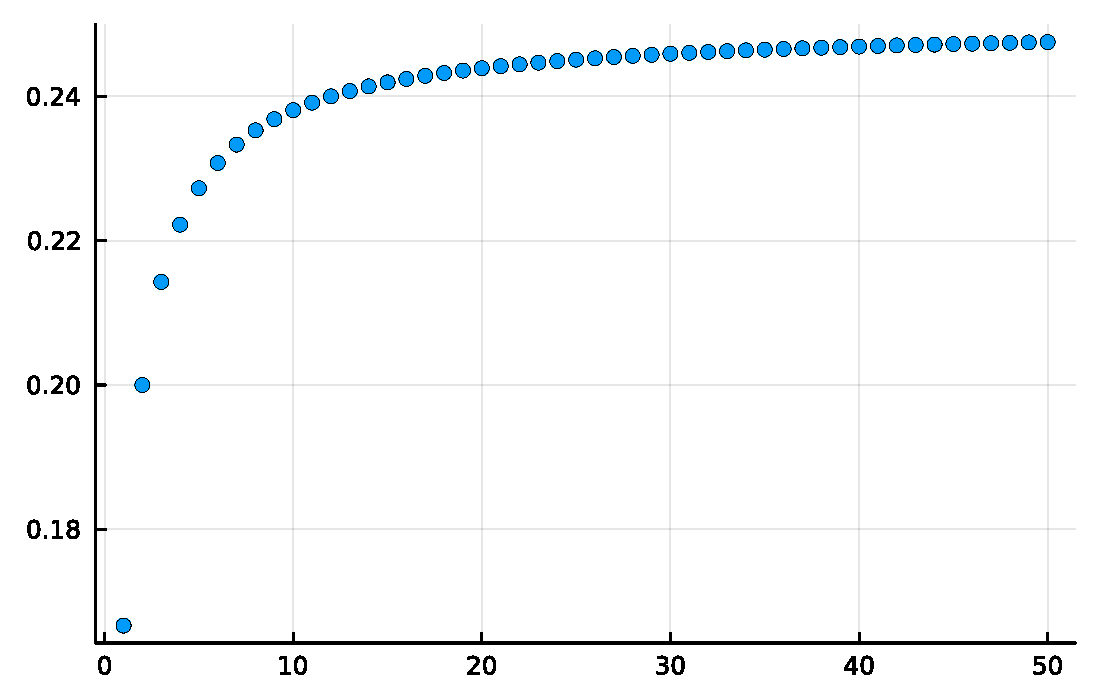
\includegraphics{./sucesiones_files/figure-pdf/cell-8-output-1.pdf}

}

\end{figure}

La sucesión converge al número \(0.25\).

\end{tcolorbox}

\begin{enumerate}
\def\labelenumi{\alph{enumi}.}
\tightlist
\item
  \(\left(\frac{2^n}{n^2}\right)_{n=1}^\infty\)
\end{enumerate}

\begin{tcolorbox}[enhanced jigsaw, arc=.35mm, toptitle=1mm, toprule=.15mm, breakable, colframe=quarto-callout-tip-color-frame, bottomtitle=1mm, titlerule=0mm, title=\textcolor{quarto-callout-tip-color}{\faLightbulb}\hspace{0.5em}{Solución}, colback=white, leftrule=.75mm, bottomrule=.15mm, rightrule=.15mm, left=2mm, colbacktitle=quarto-callout-tip-color!10!white, coltitle=black, opacitybacktitle=0.6, opacityback=0]

\begin{Shaded}
\begin{Highlighting}[]
\ImportTok{using} \BuiltInTok{Plots}
\FunctionTok{x}\NormalTok{(n) }\OperatorTok{=} \FloatTok{2}\OperatorTok{\^{}}\NormalTok{n }\OperatorTok{/}\NormalTok{ (}\FloatTok{4}\NormalTok{n }\OperatorTok{+} \FloatTok{2}\NormalTok{)}
\FunctionTok{scatter}\NormalTok{([}\FunctionTok{x}\NormalTok{(n) for n }\OperatorTok{=} \FloatTok{1}\OperatorTok{:}\FloatTok{50}\NormalTok{], legend}\OperatorTok{=}\ConstantTok{false}\NormalTok{)}
\end{Highlighting}
\end{Shaded}

\begin{figure}[H]

{\centering 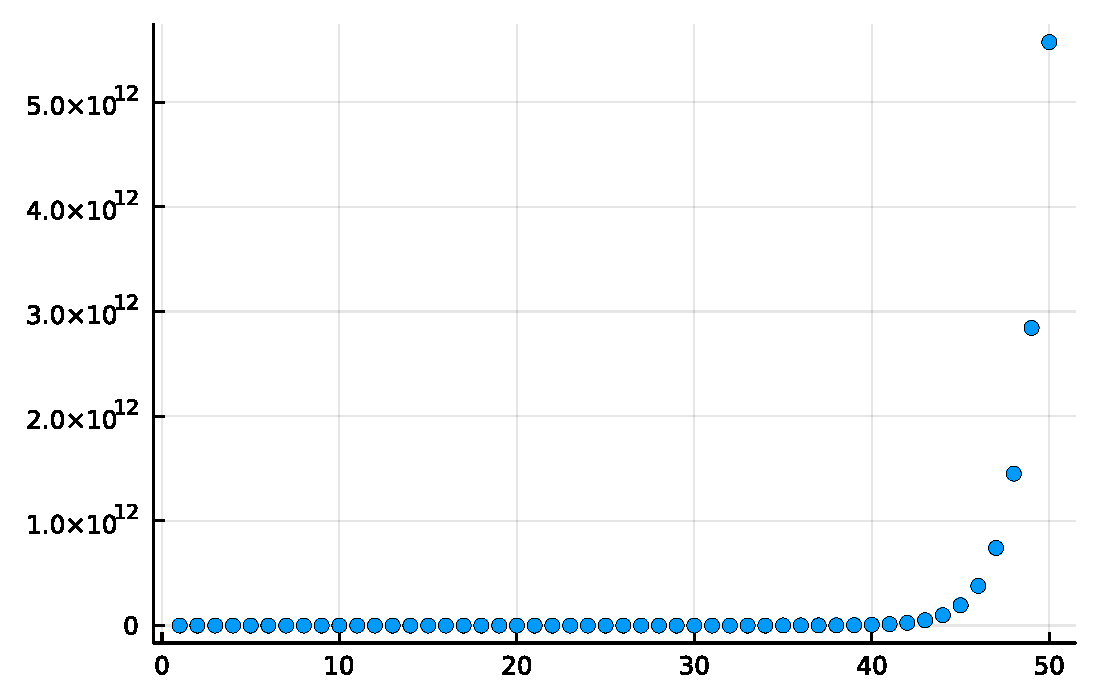
\includegraphics{./sucesiones_files/figure-pdf/cell-9-output-1.pdf}

}

\end{figure}

La sucesión diverge.

\end{tcolorbox}

\begin{enumerate}
\def\labelenumi{\alph{enumi}.}
\tightlist
\item
  \(\left(\frac{(-1)^n}{n}\right)_{n=1}^\infty\)
\end{enumerate}

\begin{tcolorbox}[enhanced jigsaw, arc=.35mm, toptitle=1mm, toprule=.15mm, breakable, colframe=quarto-callout-tip-color-frame, bottomtitle=1mm, titlerule=0mm, title=\textcolor{quarto-callout-tip-color}{\faLightbulb}\hspace{0.5em}{Solución}, colback=white, leftrule=.75mm, bottomrule=.15mm, rightrule=.15mm, left=2mm, colbacktitle=quarto-callout-tip-color!10!white, coltitle=black, opacitybacktitle=0.6, opacityback=0]

\begin{Shaded}
\begin{Highlighting}[]
\ImportTok{using} \BuiltInTok{Plots}
\FunctionTok{x}\NormalTok{(n) }\OperatorTok{=}\NormalTok{ (}\OperatorTok{{-}}\FloatTok{1}\NormalTok{)}\OperatorTok{\^{}}\NormalTok{n }\OperatorTok{/}\NormalTok{ n}
\FunctionTok{scatter}\NormalTok{([}\FunctionTok{x}\NormalTok{(n) for n }\OperatorTok{=} \FloatTok{1}\OperatorTok{:}\FloatTok{50}\NormalTok{], legend}\OperatorTok{=}\ConstantTok{false}\NormalTok{)}
\end{Highlighting}
\end{Shaded}

\begin{figure}[H]

{\centering 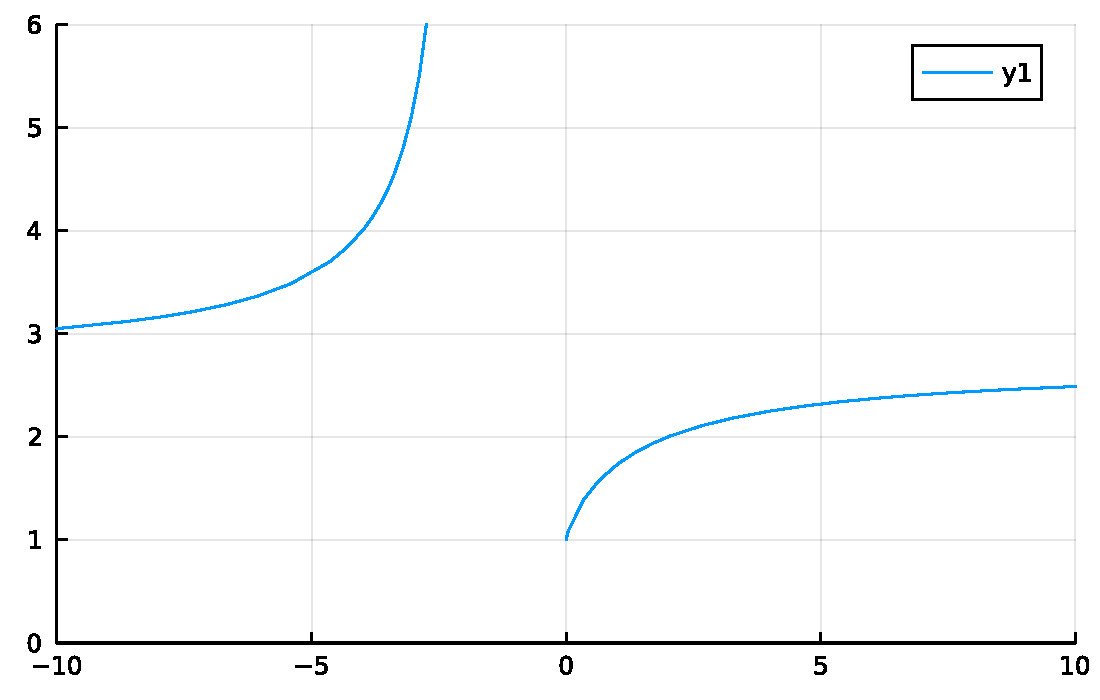
\includegraphics{./sucesiones_files/figure-pdf/cell-10-output-1.pdf}

}

\end{figure}

La sucesión converge al \(0\).

\end{tcolorbox}

\begin{enumerate}
\def\labelenumi{\alph{enumi}.}
\tightlist
\item
  \(\left(\left(1+\frac{1}{n}\right)^n\right)_{n=1}^\infty\)
\end{enumerate}

\begin{tcolorbox}[enhanced jigsaw, arc=.35mm, toptitle=1mm, toprule=.15mm, breakable, colframe=quarto-callout-tip-color-frame, bottomtitle=1mm, titlerule=0mm, title=\textcolor{quarto-callout-tip-color}{\faLightbulb}\hspace{0.5em}{Solución}, colback=white, leftrule=.75mm, bottomrule=.15mm, rightrule=.15mm, left=2mm, colbacktitle=quarto-callout-tip-color!10!white, coltitle=black, opacitybacktitle=0.6, opacityback=0]

\begin{Shaded}
\begin{Highlighting}[]
\ImportTok{using} \BuiltInTok{Plots}
\FunctionTok{x}\NormalTok{(n) }\OperatorTok{=}\NormalTok{ (}\FloatTok{1} \OperatorTok{+} \FloatTok{1} \OperatorTok{/}\NormalTok{ n)}\OperatorTok{\^{}}\NormalTok{n}
\FunctionTok{scatter}\NormalTok{([}\FunctionTok{x}\NormalTok{(n) for n }\OperatorTok{=} \FloatTok{1}\OperatorTok{:}\FloatTok{50}\NormalTok{], legend}\OperatorTok{=}\ConstantTok{false}\NormalTok{)}
\end{Highlighting}
\end{Shaded}

\begin{figure}[H]

{\centering 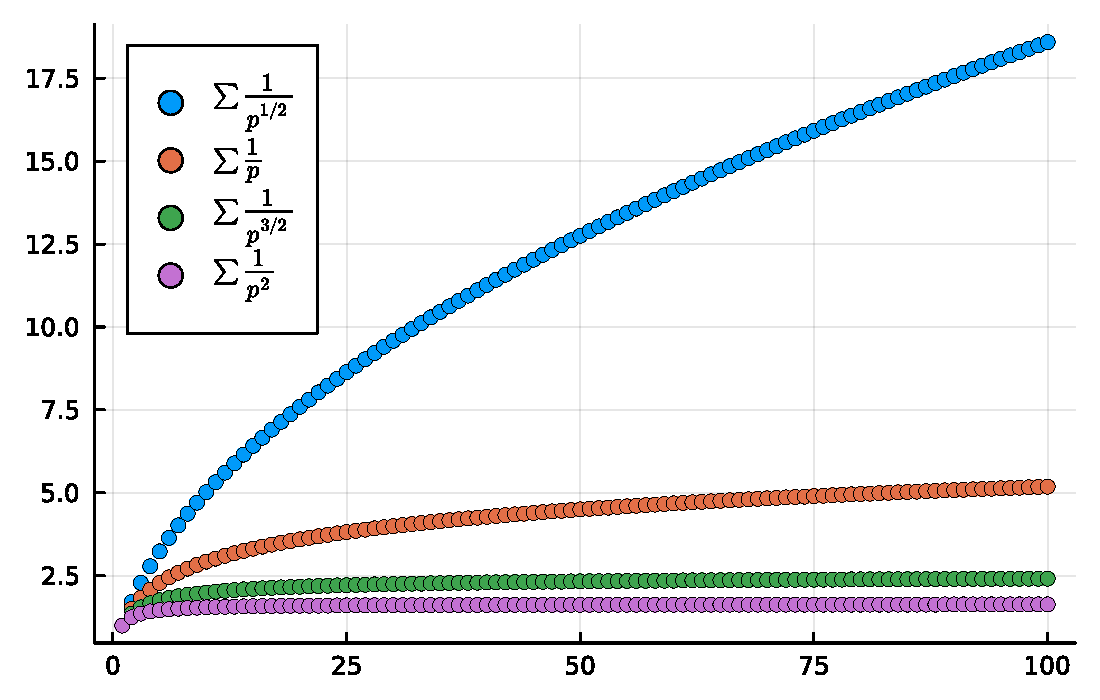
\includegraphics{./sucesiones_files/figure-pdf/cell-11-output-1.pdf}

}

\end{figure}

La sucesión converge aproximadamente a \(2.7\).

\end{tcolorbox}

\begin{enumerate}
\def\labelenumi{\alph{enumi}.}
\tightlist
\item
  \(x_1 = 2\) y \(x_{n+1}=1+\frac{1}{x_n}\) \(\forall n\in\mathbb{N}\)
\end{enumerate}

\begin{tcolorbox}[enhanced jigsaw, arc=.35mm, toptitle=1mm, toprule=.15mm, breakable, colframe=quarto-callout-tip-color-frame, bottomtitle=1mm, titlerule=0mm, title=\textcolor{quarto-callout-tip-color}{\faLightbulb}\hspace{0.5em}{Solución}, colback=white, leftrule=.75mm, bottomrule=.15mm, rightrule=.15mm, left=2mm, colbacktitle=quarto-callout-tip-color!10!white, coltitle=black, opacitybacktitle=0.6, opacityback=0]

\begin{Shaded}
\begin{Highlighting}[]
\ImportTok{using} \BuiltInTok{Plots}
\FunctionTok{x}\NormalTok{(n) }\OperatorTok{=}\NormalTok{  n }\OperatorTok{==} \FloatTok{1}\NormalTok{ ? }\FloatTok{2} \OperatorTok{:} \FloatTok{1} \OperatorTok{+} \FloatTok{1} \OperatorTok{/} \FunctionTok{x}\NormalTok{(n}\OperatorTok{{-}}\FloatTok{1}\NormalTok{)}
\FunctionTok{scatter}\NormalTok{([}\FunctionTok{x}\NormalTok{(n) for n }\OperatorTok{=} \FloatTok{1}\OperatorTok{:}\FloatTok{50}\NormalTok{], legend}\OperatorTok{=}\ConstantTok{false}\NormalTok{)}
\end{Highlighting}
\end{Shaded}

\begin{figure}[H]

{\centering 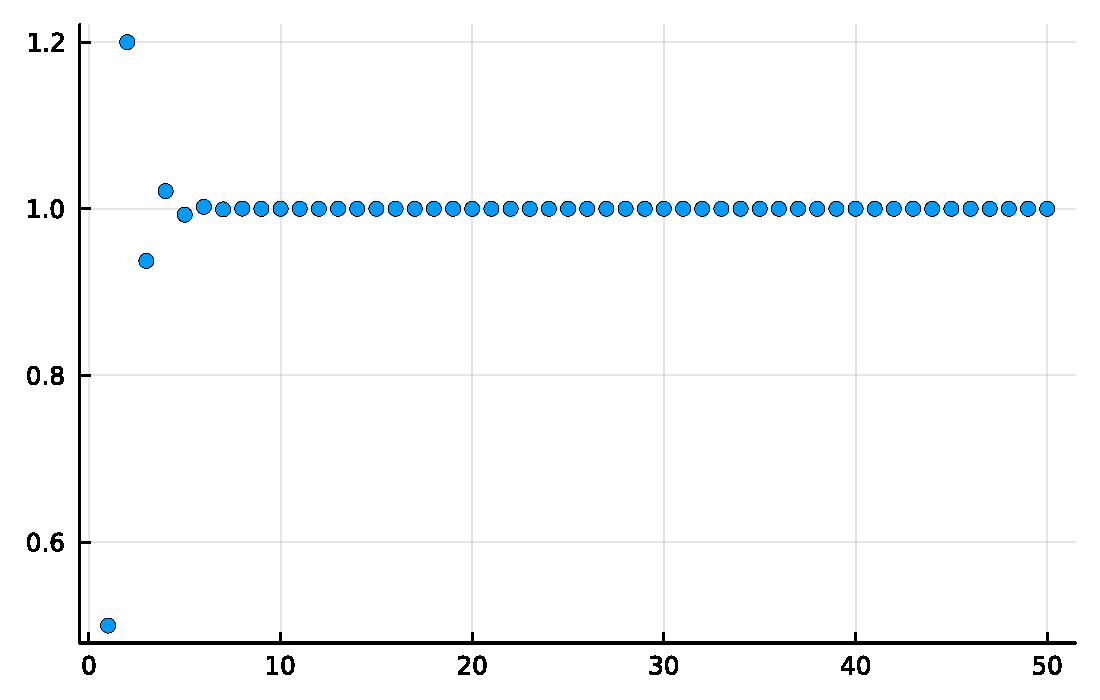
\includegraphics{./sucesiones_files/figure-pdf/cell-12-output-1.pdf}

}

\end{figure}

La sucesión converge aproximadamente a \(1.62\).

\end{tcolorbox}

\end{exercise}

\leavevmode\vadjust pre{\hypertarget{exr-limite-sucesiones}{}}%
\begin{exercise}[]\label{exr-limite-sucesiones}

Calcular el límite, si existe, de las siguiente sucesiones.

\begin{enumerate}
\def\labelenumi{\alph{enumi}.}
\tightlist
\item
  \(\left(\frac{1}{n}\right)_{n=1}^\infty\)
\end{enumerate}

\begin{tcolorbox}[enhanced jigsaw, arc=.35mm, toptitle=1mm, toprule=.15mm, breakable, colframe=quarto-callout-note-color-frame, bottomtitle=1mm, titlerule=0mm, title=\textcolor{quarto-callout-note-color}{\faInfo}\hspace{0.5em}{Pista}, colback=white, leftrule=.75mm, bottomrule=.15mm, rightrule=.15mm, left=2mm, colbacktitle=quarto-callout-note-color!10!white, coltitle=black, opacitybacktitle=0.6, opacityback=0]
Definir una función para el término general usar la función
\href{https://docs.juliahub.com/SymPy/KzewI/1.0.31/Tutorial/calculus/\#Limits-1}{\texttt{limit}}
del paquete \texttt{SymPy} para calcular el límite de la sucesión.
\end{tcolorbox}

\begin{tcolorbox}[enhanced jigsaw, arc=.35mm, toptitle=1mm, toprule=.15mm, breakable, colframe=quarto-callout-tip-color-frame, bottomtitle=1mm, titlerule=0mm, title=\textcolor{quarto-callout-tip-color}{\faLightbulb}\hspace{0.5em}{Solución}, colback=white, leftrule=.75mm, bottomrule=.15mm, rightrule=.15mm, left=2mm, colbacktitle=quarto-callout-tip-color!10!white, coltitle=black, opacitybacktitle=0.6, opacityback=0]

\begin{Shaded}
\begin{Highlighting}[]
\ImportTok{using} \BuiltInTok{SymPy}
\PreprocessorTok{@syms}\NormalTok{ n}\OperatorTok{::}\DataTypeTok{(integer}\NormalTok{, positive)  }\CommentTok{\# Declaración de la variable simbólica n.}
\FunctionTok{x}\NormalTok{(n) }\OperatorTok{=} \FloatTok{1}\OperatorTok{/}\NormalTok{n}
\FunctionTok{limit}\NormalTok{(}\FunctionTok{x}\NormalTok{(n), n}\OperatorTok{=\textgreater{}}\NormalTok{oo)}
\end{Highlighting}
\end{Shaded}

$0$

\end{tcolorbox}

\begin{enumerate}
\def\labelenumi{\alph{enumi}.}
\setcounter{enumi}{2}
\tightlist
\item
  \(\left((-1)^n\right)_{n=1}^\infty\)
\end{enumerate}

\begin{tcolorbox}[enhanced jigsaw, arc=.35mm, toptitle=1mm, toprule=.15mm, breakable, colframe=quarto-callout-tip-color-frame, bottomtitle=1mm, titlerule=0mm, title=\textcolor{quarto-callout-tip-color}{\faLightbulb}\hspace{0.5em}{Solución}, colback=white, leftrule=.75mm, bottomrule=.15mm, rightrule=.15mm, left=2mm, colbacktitle=quarto-callout-tip-color!10!white, coltitle=black, opacitybacktitle=0.6, opacityback=0]

\begin{Shaded}
\begin{Highlighting}[]
\PreprocessorTok{@syms}\NormalTok{ n}\OperatorTok{::}\DataTypeTok{(integer}\NormalTok{, positive)}
\FunctionTok{x}\NormalTok{(n) }\OperatorTok{=}\NormalTok{ (}\OperatorTok{{-}}\FloatTok{1}\NormalTok{)}\OperatorTok{\^{}}\NormalTok{n}
\FunctionTok{limit}\NormalTok{(}\FunctionTok{x}\NormalTok{(n), n}\OperatorTok{=\textgreater{}}\NormalTok{oo)}
\end{Highlighting}
\end{Shaded}

$\text{NaN}$

\end{tcolorbox}

\begin{enumerate}
\def\labelenumi{\alph{enumi}.}
\setcounter{enumi}{3}
\tightlist
\item
  \(\left(\left(1+\frac{1}{n}\right)^n\right)_{n=1}^\infty\)
\end{enumerate}

\begin{tcolorbox}[enhanced jigsaw, arc=.35mm, toptitle=1mm, toprule=.15mm, breakable, colframe=quarto-callout-tip-color-frame, bottomtitle=1mm, titlerule=0mm, title=\textcolor{quarto-callout-tip-color}{\faLightbulb}\hspace{0.5em}{Solución}, colback=white, leftrule=.75mm, bottomrule=.15mm, rightrule=.15mm, left=2mm, colbacktitle=quarto-callout-tip-color!10!white, coltitle=black, opacitybacktitle=0.6, opacityback=0]

\begin{Shaded}
\begin{Highlighting}[]
\PreprocessorTok{@syms}\NormalTok{ n}\OperatorTok{::}\DataTypeTok{(integer}\NormalTok{, positive)}
\FunctionTok{x}\NormalTok{(n) }\OperatorTok{=}\NormalTok{ (}\FloatTok{1} \OperatorTok{+} \FloatTok{1} \OperatorTok{/}\NormalTok{ n)}\OperatorTok{\^{}}\NormalTok{n}
\FunctionTok{limit}\NormalTok{(}\FunctionTok{x}\NormalTok{(n), n}\OperatorTok{=\textgreater{}}\NormalTok{oo)}
\end{Highlighting}
\end{Shaded}

$e$

\end{tcolorbox}

\end{exercise}

\leavevmode\vadjust pre{\hypertarget{exr-calculo-pi}{}}%
\begin{exercise}[]\label{exr-calculo-pi}

En el siglo III A.C
\href{https://es.wikipedia.org/wiki/Arqu\%C3\%ADmedes}{Arquímedes} usó
el
\href{https://es.wikipedia.org/wiki/M\%C3\%A9todo_por_agotamiento}{método
por agotamiento} para calcular el área encerrada por una circunferencia
(y de paso el valor de \(\pi\)). La idea consiste en inscribir la
circunferencia en polígonos regulares con un número de lados cada vez
mayor.

\begin{figure}

{\centering 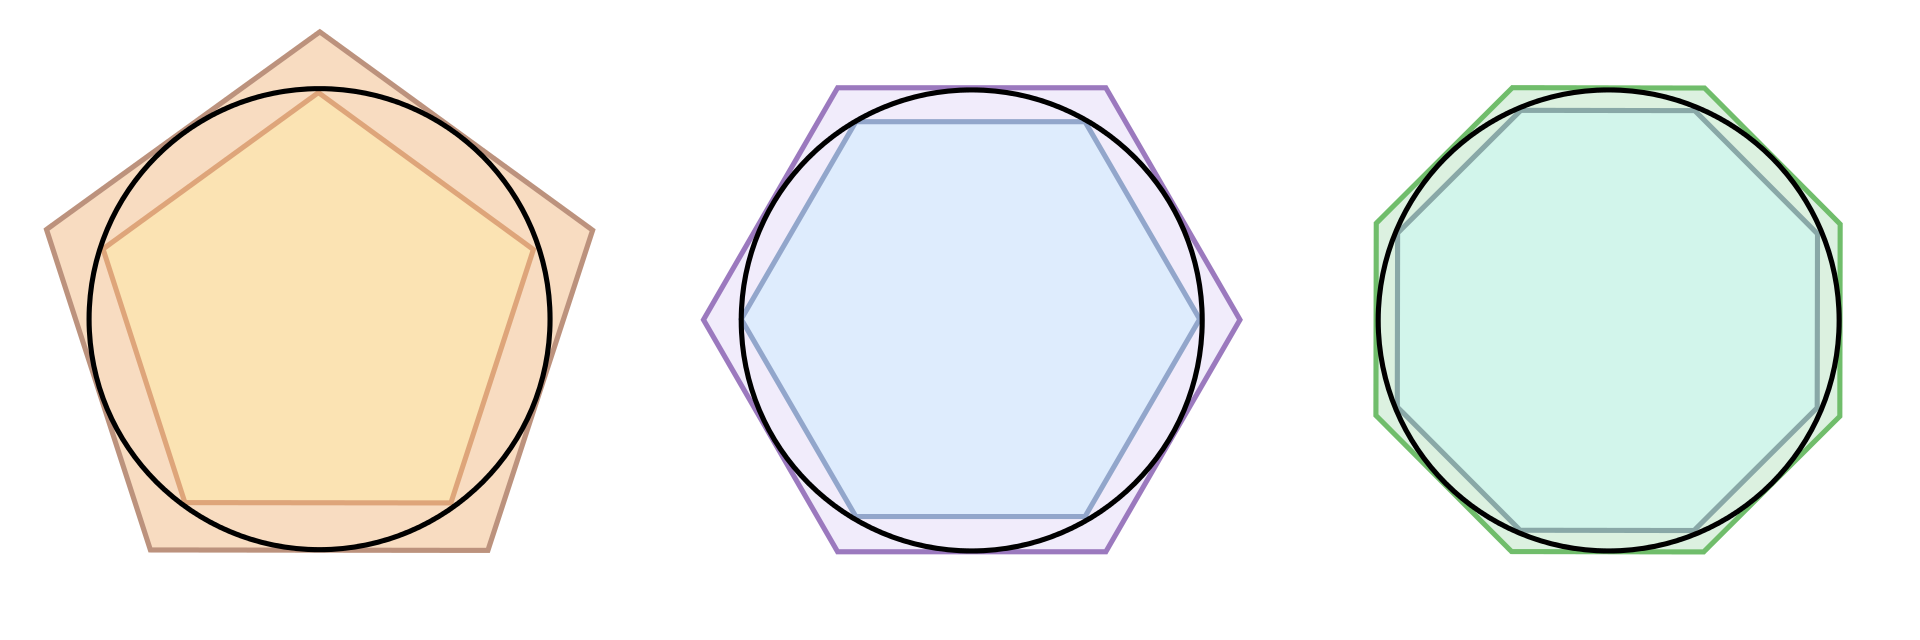
\includegraphics{./img/sucesiones/poligonos-circunferencia.png}

}

\caption{Aproximación del área de una circunferencia mediante polígonos
regulares}

\end{figure}

El área de estos polígonos puede calcularse fácilmente descomponiendo
los polígonos regulares en triángulos como en el siguiente ejemplo.

\begin{figure}

{\centering 

\usetikzlibrary{shapes.geometric}
\usetikzlibrary{angles}
\definecolor{myblue}{rgb}{0.067,0.529,0.871}
\definecolor{mypurple}{rgb}{0.859,0.071,0.525}
\definecolor{myred}{rgb}{1.0, 0.13, 0.32}
\definecolor{mygreen}{rgb}{0.01, 0.75, 0.24}
\def\PolyRadius{2cm}
\begin{tikzpicture}[draw=myblue, text=myblue]
\draw (0,0) circle (2);
\coordinate (A) at (-1,-1.74);
\coordinate (B) at (0,0);
\coordinate (C) at (1,-1.74);
\fill[fill=red!20] (0,0) -- (-1,-1.74) -- (1, -1.74) -- (0,0);
\node[regular polygon,draw,regular polygon sides = 6,minimum size=2*\PolyRadius] at (0,0) {};
\draw pic[draw,angle radius=0.5cm]{angle=A--B--C};
\node at (0,-0.35) {\scriptsize $\alpha$};
\draw [dashed] (0,0) -- (2,0);
\draw [dashed] (0,0) -- (-2,0);
\draw [dashed] (0,0) -- (1,1.74);
\draw [dashed] (0,0) -- (-1,1.74);
\draw [dashed] (0,0) -- (-1,-1.74);
\draw [dashed] (0,0) -- (1,-1.74) node[right, midway] {$r$};
\end{tikzpicture}


}

\caption{Descomposición de un hexágono en triángulos}

\end{figure}

En el caso de los polígonos inscritos dentro de la circunferencia, como
dos de los lados siempre coinciden con el radio de la circunferencia
\(r\), el área del polígono de \(n\) lados puede calcularse con la
fórmula

\[
a_n = \frac{1}{2}nr^2\operatorname{sen}\left(\frac{360}{n}\right)
\]

\begin{enumerate}
\def\labelenumi{\alph{enumi}.}
\tightlist
\item
  Calcular el área de los polígonos de \(10^i\) lados, para
  \(i=1,\ldots, 6\) tomando \(r=1\).
\end{enumerate}

\begin{tcolorbox}[enhanced jigsaw, arc=.35mm, toptitle=1mm, toprule=.15mm, breakable, colframe=quarto-callout-tip-color-frame, bottomtitle=1mm, titlerule=0mm, title=\textcolor{quarto-callout-tip-color}{\faLightbulb}\hspace{0.5em}{Solución}, colback=white, leftrule=.75mm, bottomrule=.15mm, rightrule=.15mm, left=2mm, colbacktitle=quarto-callout-tip-color!10!white, coltitle=black, opacitybacktitle=0.6, opacityback=0]

\begin{Shaded}
\begin{Highlighting}[]
\FunctionTok{a}\NormalTok{(n) }\OperatorTok{=} \FunctionTok{n*sind}\NormalTok{(}\FloatTok{360}\OperatorTok{/}\NormalTok{n)}\OperatorTok{/}\FloatTok{2}
\FunctionTok{print}\NormalTok{([}\FunctionTok{a}\NormalTok{(}\FloatTok{10}\OperatorTok{\^{}}\NormalTok{i) for i }\OperatorTok{=} \FloatTok{1}\OperatorTok{:}\FloatTok{6}\NormalTok{])}
\end{Highlighting}
\end{Shaded}

\begin{verbatim}
[2.938926261462366, 3.1395259764656687, 3.1415719827794755, 3.141592446881286, 3.141592651522708, 3.1415926535691225]
\end{verbatim}

\end{tcolorbox}

\begin{enumerate}
\def\labelenumi{\alph{enumi}.}
\setcounter{enumi}{1}
\tightlist
\item
  Dibujar con los primeros 50 términos de la sucesión de las areas de
  los polígonos tomando \(r=1\).
\end{enumerate}

\begin{tcolorbox}[enhanced jigsaw, arc=.35mm, toptitle=1mm, toprule=.15mm, breakable, colframe=quarto-callout-tip-color-frame, bottomtitle=1mm, titlerule=0mm, title=\textcolor{quarto-callout-tip-color}{\faLightbulb}\hspace{0.5em}{Solución}, colback=white, leftrule=.75mm, bottomrule=.15mm, rightrule=.15mm, left=2mm, colbacktitle=quarto-callout-tip-color!10!white, coltitle=black, opacitybacktitle=0.6, opacityback=0]

\begin{Shaded}
\begin{Highlighting}[]
\ImportTok{using} \BuiltInTok{Plots}
\FunctionTok{a}\NormalTok{(n) }\OperatorTok{=} \FunctionTok{n*sind}\NormalTok{(}\FloatTok{360}\OperatorTok{/}\NormalTok{n)}\OperatorTok{/}\FloatTok{2}
\FunctionTok{scatter}\NormalTok{([}\FunctionTok{a}\NormalTok{(n) for n }\OperatorTok{=} \FloatTok{1}\OperatorTok{:}\FloatTok{50}\NormalTok{], legend}\OperatorTok{=}\ConstantTok{false}\NormalTok{)}
\end{Highlighting}
\end{Shaded}

\begin{figure}[H]

{\centering 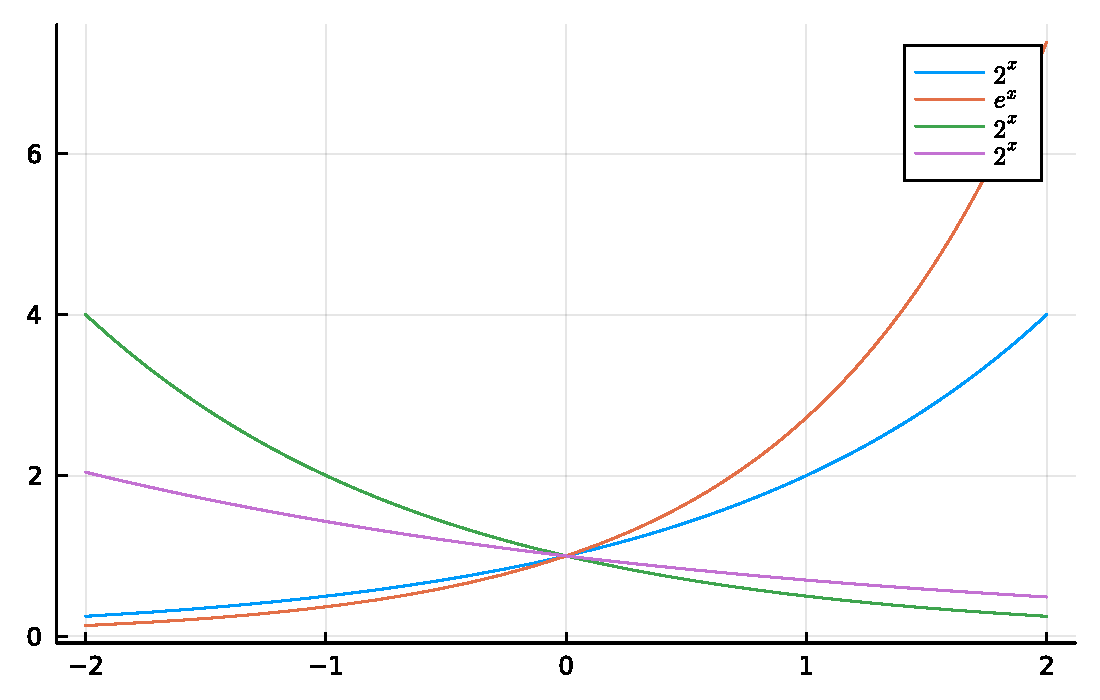
\includegraphics{./sucesiones_files/figure-pdf/cell-17-output-1.pdf}

}

\end{figure}

\end{tcolorbox}

\begin{enumerate}
\def\labelenumi{\alph{enumi}.}
\setcounter{enumi}{2}
\tightlist
\item
  Calcular el límite de la sucesión de las areas de los polígonos
  tomando \(r=1\).
\end{enumerate}

\begin{tcolorbox}[enhanced jigsaw, arc=.35mm, toptitle=1mm, toprule=.15mm, breakable, colframe=quarto-callout-tip-color-frame, bottomtitle=1mm, titlerule=0mm, title=\textcolor{quarto-callout-tip-color}{\faLightbulb}\hspace{0.5em}{Solución}, colback=white, leftrule=.75mm, bottomrule=.15mm, rightrule=.15mm, left=2mm, colbacktitle=quarto-callout-tip-color!10!white, coltitle=black, opacitybacktitle=0.6, opacityback=0]

\begin{Shaded}
\begin{Highlighting}[]
\ImportTok{using} \BuiltInTok{SymPy}
\PreprocessorTok{@syms}\NormalTok{ n}\OperatorTok{::}\DataTypeTok{(integer}\NormalTok{, positive)}
\FunctionTok{a}\NormalTok{(n) }\OperatorTok{=} \FunctionTok{n*sin}\NormalTok{(}\FloatTok{2}\NormalTok{pi}\OperatorTok{/}\NormalTok{n)}\OperatorTok{/}\FloatTok{2}
\FunctionTok{limit}\NormalTok{(}\FunctionTok{a}\NormalTok{(n), n}\OperatorTok{=\textgreater{}}\NormalTok{oo)}
\end{Highlighting}
\end{Shaded}

$3.14159265358979$

\end{tcolorbox}

\begin{enumerate}
\def\labelenumi{\alph{enumi}.}
\setcounter{enumi}{3}
\tightlist
\item
  Usando el resultado anterior, calcular el area del círculo de radio
  \(r\).
\end{enumerate}

\begin{tcolorbox}[enhanced jigsaw, arc=.35mm, toptitle=1mm, toprule=.15mm, breakable, colframe=quarto-callout-tip-color-frame, bottomtitle=1mm, titlerule=0mm, title=\textcolor{quarto-callout-tip-color}{\faLightbulb}\hspace{0.5em}{Solución}, colback=white, leftrule=.75mm, bottomrule=.15mm, rightrule=.15mm, left=2mm, colbacktitle=quarto-callout-tip-color!10!white, coltitle=black, opacitybacktitle=0.6, opacityback=0]

\begin{Shaded}
\begin{Highlighting}[]
\ImportTok{using} \BuiltInTok{SymPy}
\PreprocessorTok{@syms}\NormalTok{ n}\OperatorTok{::}\DataTypeTok{(integer}\NormalTok{, positive), r}
\FunctionTok{a}\NormalTok{(n) }\OperatorTok{=}\NormalTok{ n}\OperatorTok{*}\NormalTok{r}\OperatorTok{\^{}}\FloatTok{2}\FunctionTok{*sin}\NormalTok{(}\FloatTok{2}\NormalTok{pi}\OperatorTok{/}\NormalTok{n)}\OperatorTok{/}\FloatTok{2}
\FunctionTok{limit}\NormalTok{(}\FunctionTok{a}\NormalTok{(n), n}\OperatorTok{=\textgreater{}}\NormalTok{oo)}
\end{Highlighting}
\end{Shaded}

$3.14159265358979 r^{2}$

\end{tcolorbox}

\end{exercise}

\hypertarget{ejercicios-propuestos}{%
\section{Ejercicios propuestos}\label{ejercicios-propuestos}}

\leavevmode\vadjust pre{\hypertarget{exr-sucesiones-propuesto-1}{}}%
\begin{exercise}[]\label{exr-sucesiones-propuesto-1}

Calcular el décimo término de la sucesión
\(\left(\frac{3n^2+n}{6n^2-1}\right)_{n=1}^\infty\).

\vspace{18pt}*Hint: *

Introducir hasta 5 decimales

\end{exercise}

\leavevmode\vadjust pre{\hypertarget{exr-sucesiones-propuesto-2}{}}%
\begin{exercise}[]\label{exr-sucesiones-propuesto-2}

Calcular los 10 primeros términos de la sucesión
\(\left(\frac{3n^2+n}{6n^2-1}\right)_{n=1}^\infty\) y averiguar hacia
dónde converge.

${\quad\Box}$ 1

${\quad\Box}$ 0.5

${\quad\Box}$ No converge

${\quad\Box}$ 0

${\quad\Box}$ 1.5

\end{exercise}

\leavevmode\vadjust pre{\hypertarget{exr-sucesiones-propuesto-3}{}}%
\begin{exercise}[]\label{exr-sucesiones-propuesto-3}

¿Cuál de las siguientes gráficas corresponde a la sucesión \(x_1=3\) y
\(x_{n+1}=\sqrt{2x_n}\) \(\forall n=2,3,\ldots\).

insert image here

\end{exercise}

\leavevmode\vadjust pre{\hypertarget{exr-sucesiones-propuesto-4}{}}%
\begin{exercise}[]\label{exr-sucesiones-propuesto-4}

A la vista de la gráfica de los 20 primeros términos de la sucesión
\(\left(\frac{2^n}{n!}\right)_{n=1}^\infty\), ¿crees que la sucesión
converge?

${\quad\Box}$ Si

${\quad\Box}$ No

\end{exercise}

\leavevmode\vadjust pre{\hypertarget{exr-sucesiones-propuesto-5}{}}%
\begin{exercise}[]\label{exr-sucesiones-propuesto-5}

A la vista de la gráfica de los 10 primeros términos de la sucesión
\(\left(\frac{n^n}{n!}\right)_{n=1}^\infty\), ¿crees que la sucesión
converge?

${\quad\Box}$ Si

${\quad\Box}$ No

\end{exercise}

\leavevmode\vadjust pre{\hypertarget{exr-sucesiones-propuesto-6}{}}%
\begin{exercise}[]\label{exr-sucesiones-propuesto-6}

A la vista de la gráfica de los 20 primeros términos de la sucesión dada
por \(x_1=1\) y \(x_{n+1}=\sqrt{x_n+2}\) \(\forall n\in \mathbb{N}\),
¿crees que la sucesión converge?

${\quad\Box}$ Si

${\quad\Box}$ No

\end{exercise}

\leavevmode\vadjust pre{\hypertarget{exr-sucesiones-propuesto-7}{}}%
\begin{exercise}[]\label{exr-sucesiones-propuesto-7}

¿Cuál es el límite de la sucesión
\(\left(\left(1+\frac{2}{n}\right)^n\right)_{n=1}^\infty\)

\vspace{18pt}*Hint: *

Introducir hasta 5 decimales

\end{exercise}



\end{document}
